%Results

\subsection{Theraulaz Model}
\subsubsection*{Division of labour}
Our model is able to simulate the divison of labour. In Fig.\ref{fig:thetax} on the left we see the development of the thresholds $\theta_{ij}$ as a function of time. For each individuum $i$ there is one line with respect to each task $j$. Here, we have used N=5 bees and M=2 tasks, amounting to 10 depicted lines - one line for each task for each bee. We can see that in the beginning the values of $\theta_{ij}$ oscillate and then assume a steady state from approximately $t=3000$ on. In this steady state, exactly five lines assume the constant maximum value $\theta_{ij}=1000$ and five lines assume the constant minimum value $\theta_{ij}=0$. This means that the five bees specialize in exactly one task and keep performing this single task in the steady state.

\begin{figure}[ht!]
	\centering
	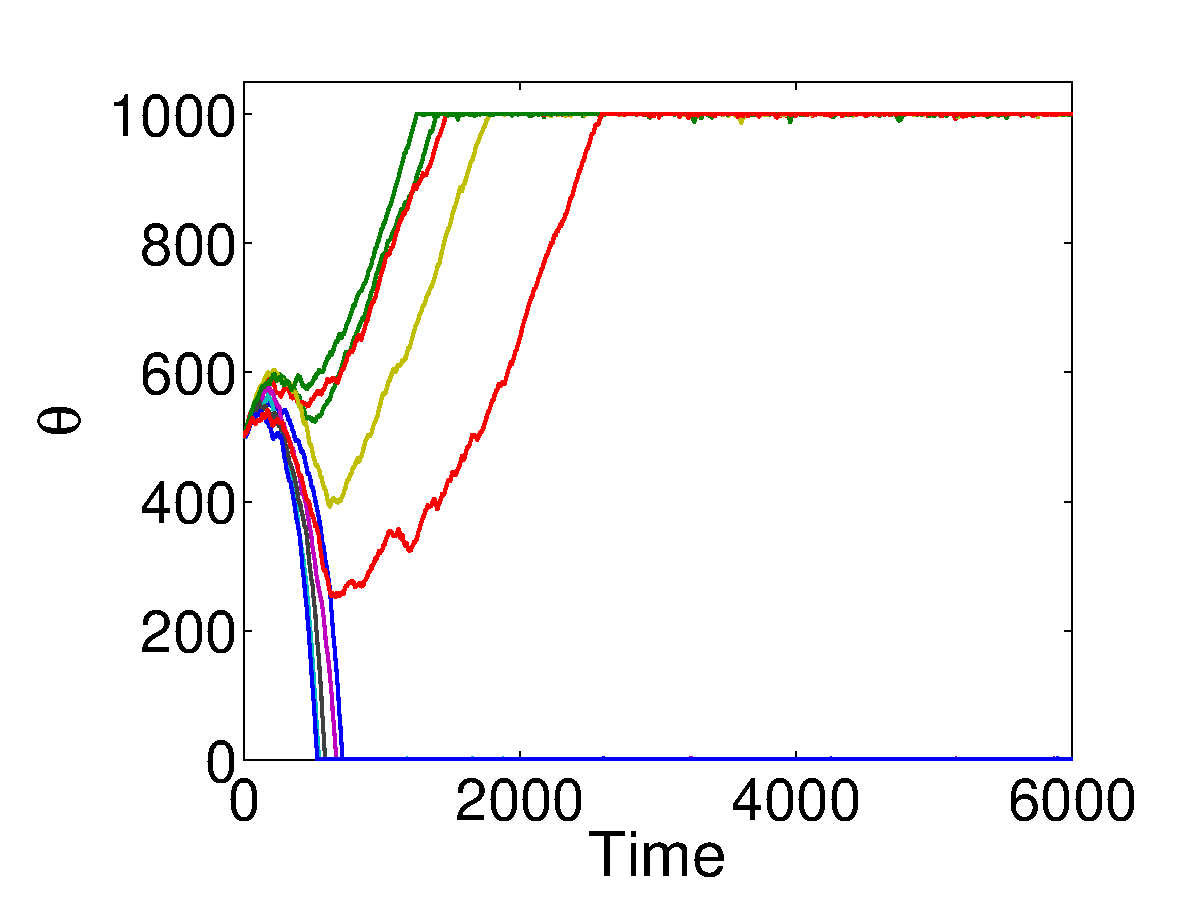
\includegraphics[width=0.4\textwidth]{figures/thetax.eps}
	\caption{$\theta$ as a function of time.}
	\label{fig:thetax}
\end{figure}

This behaviour can be explained as follows. In the beginning, the five bees have no preference for any task as their $\theta=500$ for all tasks. In other words, there is no specialization yet. First, a bee tries out to perform one of the two tasks and gets inactive with a certain probability over time. It might subsequently decide to continue pursuing its first task or alternatively perform the second one. This decision is influenced by two factors. First, by the choice of the other bees. If all bees perform task 1, the stimulus for this task will be negligible compared to the increasing stimulus for task 2 and it becomes more likely to perform this second task. Second, by the skills the bee has gained or forgotten with respect to a specific task. The more time a bee spends pursuing task 1, the better it gets performing it. In our model, the bee is then more likely to continue pursuing this task. Vice versa is true for a task which is not performed regularly by a bee. Therefore, what we observe is that some bees will exclusively perform task 1, thus $\theta_{j=1}=0$ and $\theta_{j=2}=1000$ in the steady state, and others decide to perform task 2, thus $\theta_{j=2}=0$ and $\theta_{j=1}=1000$. The model consequently allows for the investigation of the division of labour in societies. Driving force for the division is the specialization by a learning and forgetting process.
In Fig.\ref{fig:thetax}  on the right we can see x as a function of time.

\subsubsection{Measurement of the development and performance of a society}
Our model enables the description of the performance of the bee hive. In Fig.\ref{fig:welstim} the thresholds, the corresponding stimuli with respect to task $j=1, 2$ as well as the corresponding total welfare W of the society is depicted. The behaviour of the thresholds is analogous to what is already described in Fig.\ref{fig:thetax}. The corresponding stimuli increase in time, reach a maximum value at approximately time=500 and subsequently decrease to zero. Remarkably, the stimulus of task 2 decreases slower than that of task 1. The development of the welfare curve is closely related to the development of the stimuli. At times the stimuli are high the welfare is low. Thus, the welfare first decreases, goes through a minimum at approximately time=500 and then slowly increases to reach its maximum value of 1. Note that in all graphs all functions reach its steady state value at approximately time=3000.

\begin{figure}[ht!]
	\centerline{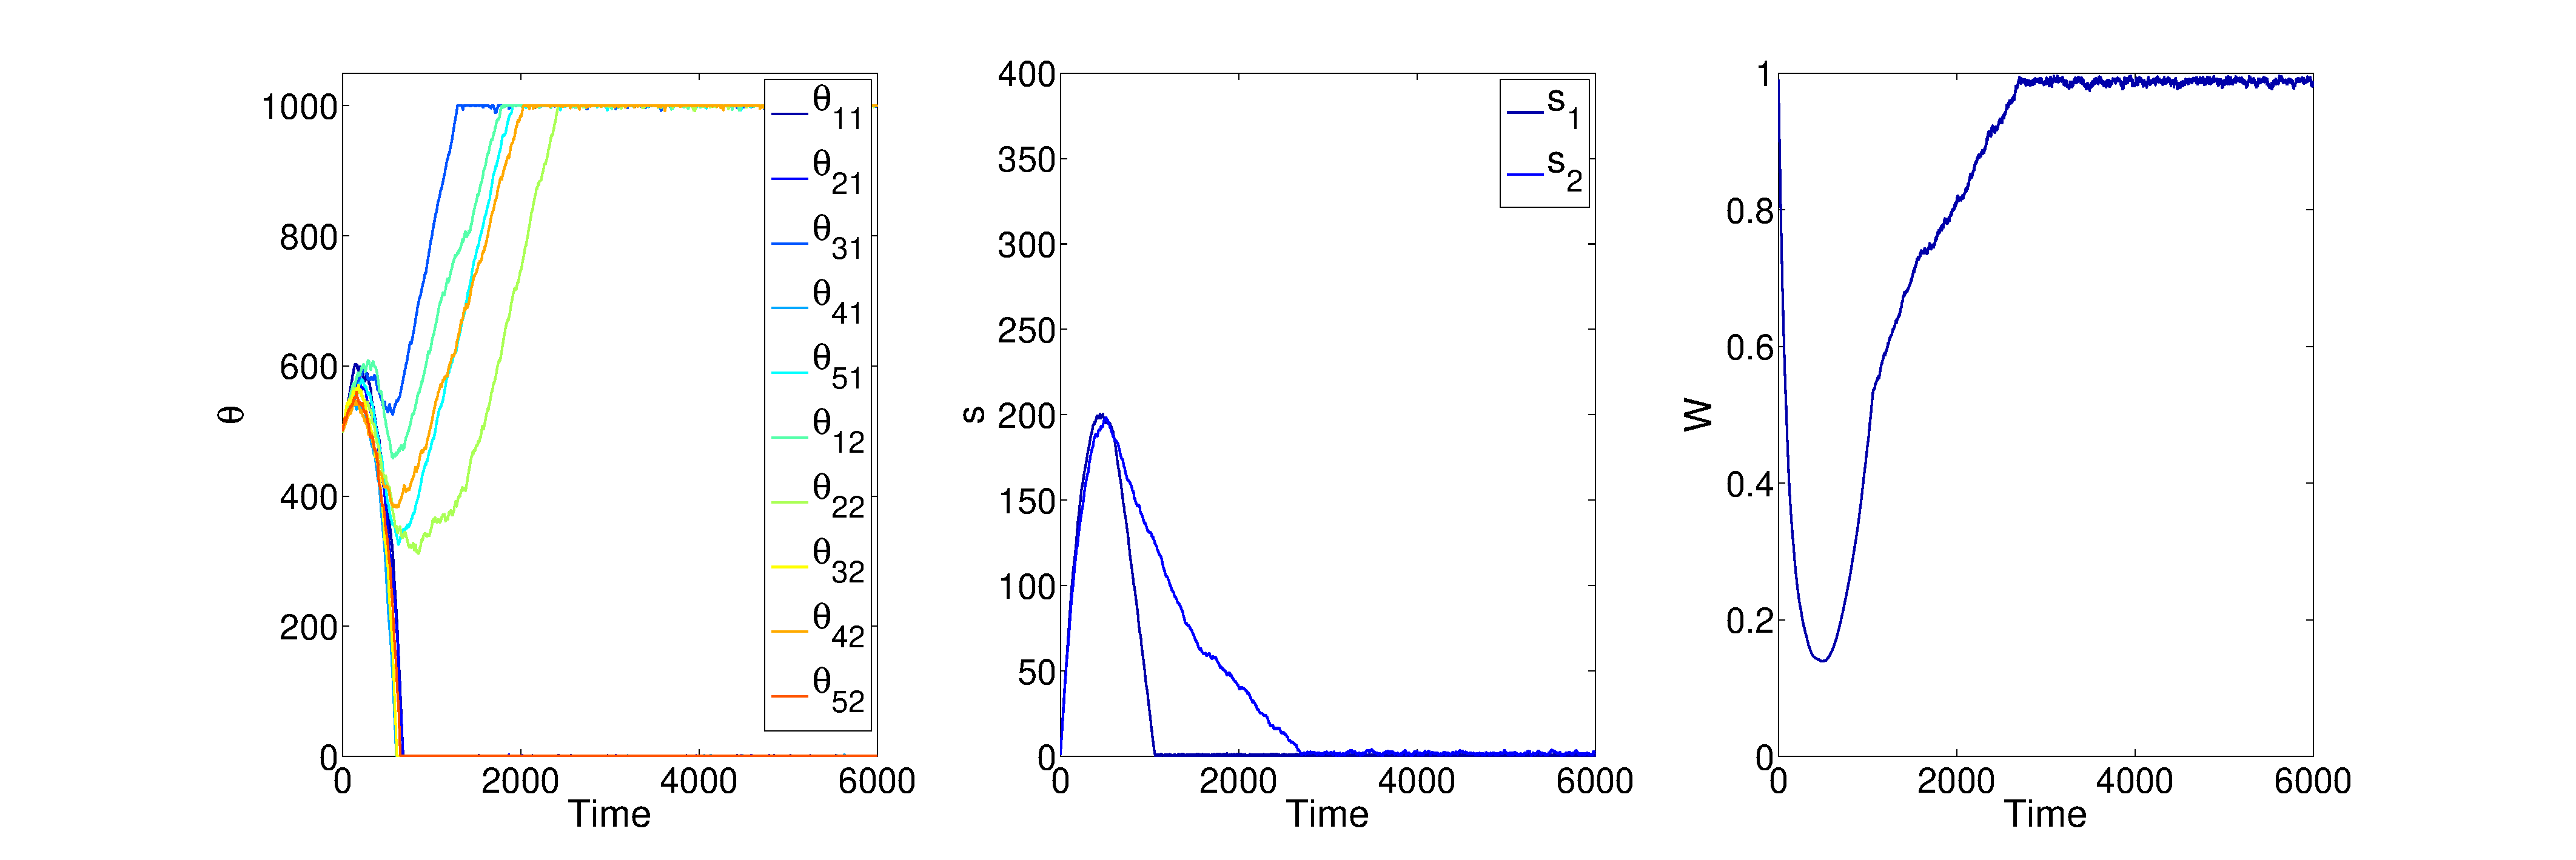
\includegraphics[width=1.25\textwidth]{figures/welstim.eps}}
	
	\caption{Left: Tresholds $\theta$ as a function of time. Middle: Stimuli $s_{j}$ for task 1 and two as a function of time. Right: Welfare W as a function of time.}
	\label{fig:welstim}
\end{figure}

The functions can be interpreted as follows. The development of the stimuli can be explained by the fact that it takes time for the bees to reach an equilibrium state -- the state where all bees assume exactly one task. Up to this point, the needs of the hive are not sufficiently satisfied. Hence, the stimuli increase. Over time, the bees become more specialized towards a specific task and the stimuli go through a maximum to decrease subsequently. This is an expression that the tasks are performed with a sufficient efficiency. The individual development of the thresholds and stimuli is governed by how fast the bees manage to specialize themselves and satisfy the need for the respective task. In the presented case, for example, one can look at the stimulus and the threshold value which converge last to their equilibrium value - stimulus 2 and threshold $\theta_{22}$. Stimulus 2 decreases slower than stimulus 1, so the need to perform 2 is greater for a longer period of time compared to task 1. This is reflected in the curve of $\theta_{22}$. It remains low as long as stimulus 2 is high and only then converges to 1000. This means that bee 2 engages as long in task 2 as stimulus 2 remains high. Thereafter it becomes inactive with respect to task 2 and is thus the last bee to be fully specialized. The welfare is connected to the sum of the stimuli. The stimuli are high when the hive need that specific tasks need to be performed in order for the hive to survive. Whenever a task is not performed, or to an insufficient extent, the respective stimulus is high. High stimuli thus reflect a poor state. Vice versa, low stimuli show that the hive performs well. Therefore, we have introduced the welfare model which is based on the sum of the stimuli. When the sum of the stimuli is low, indicating a good performance of the hive, the welfare increases. Hence, our model is able to describe how well specific tasks are performed and to measure the total welfare of a population over time.

\subsubsection{Perturbations}
Model 1 has been analyzed with respect to an isolated society. It has been used to describe domestic characteristics of a society, such as division of labour and welfare. However, we also want to investigate how the model can be used to describe external disturbances, where the work environment is changed or individuals can get killed (or are otherwise removed). Therefore, we have studied the response of the model with respect to perturbations such as reinitializing either a random bee, or every bee or every bee perform a same task.
In the following, we will consider the special case in which the colony consists of five bees and two tasks. Before starting a deep analysis, it is important to know that for this specific setup the bees usually reach an equilibrium state in which two bees work on a task and the three others work on the other task. 

\paragraph{Reinitializing one bee}
Let us initially assume that the model has reached an equilibrium before being subject to a perturbation. We will start with a simple case: reset the associated features $x_{ij}$ and $\theta{ij}$ of a single bee. Here, we need to consider two cases. First, the removed bee was working on the task performed by only a single other bee. Second, the removed bee was performing its task together with two other bees.

In Fig.\ref{fig:figure1} $\theta{ij}$ and $x_{ij}$ of all bees are shown as a function of time. During this time, we have randomly reinitiated a single bee at approximately 2300, 3900 and 7200 iterations. This can be seen at the discontinuities for the corresponding $\theta{ij}$ and $x_{ij}$ graphs. To study case 1, we can look at the perturbation at 3900 iterations, as indicated by an arrow. Here, bee three was reinitialized, thus $x_{i=3,j}=0$ and $\theta{i=3,j}=500$. As one can see the $x_{ij}$ and $\theta{ij}$ values for all other bees remain unaffected. The $\theta{i=3,j}$ and $x_{i=3,j}=0$ values of bee three are reset but converge to their initital values again. This means that for case one the system is robust in the sense that the same equilibrium is reached as prior to the disturbance. The unaffected bees continue to work and the reinitialized bee returns to its initial work again.

\begin{figure}[ht!]
	\centering
	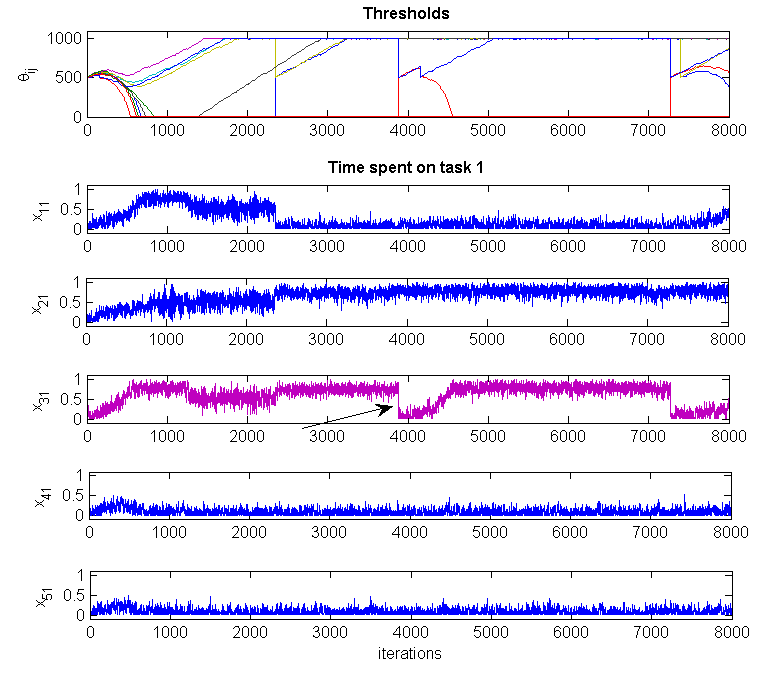
\includegraphics[width=0.8\textwidth]{figures/figure1}
	\caption{Reinitializing a bee working on a task fulfilled by only one other bee after 3900 iterations.}
	\label{fig:figure1}
\end{figure}

For the second case, we can look at the reinitialization taking place at 2300 iterations. In this case a bee ($i=1$) was removed, which was working together with two other bees ($i=2,3$) on a single task. We observe that $x_{i=2,3,j}$ increase after removing bee one. The corresponding values for bee 4 and 5 remain unaffected, however. Subsequently, the reinitialized bee

This implies that the former partners of bee 1 step up and work more intensively.

In the second case, there are still two other workers left to do the task initially performed by our reinitialized bee. These two bees instantaneously step up and start working more than they used to in order to compensate the loss induced by the reset. Since each task is now carried out by two bees, our reset bee is not inclined to work anymore. The given stimuli are not sufficiently high. In this case, we reach a new equilibrium, where each task is performed by two bees and the fifth bee is inactive. This transition from one equilibrium to another one has different consequences which will be examined in the following.

\begin{center}
\begin{figure}[ht!]
\centering{}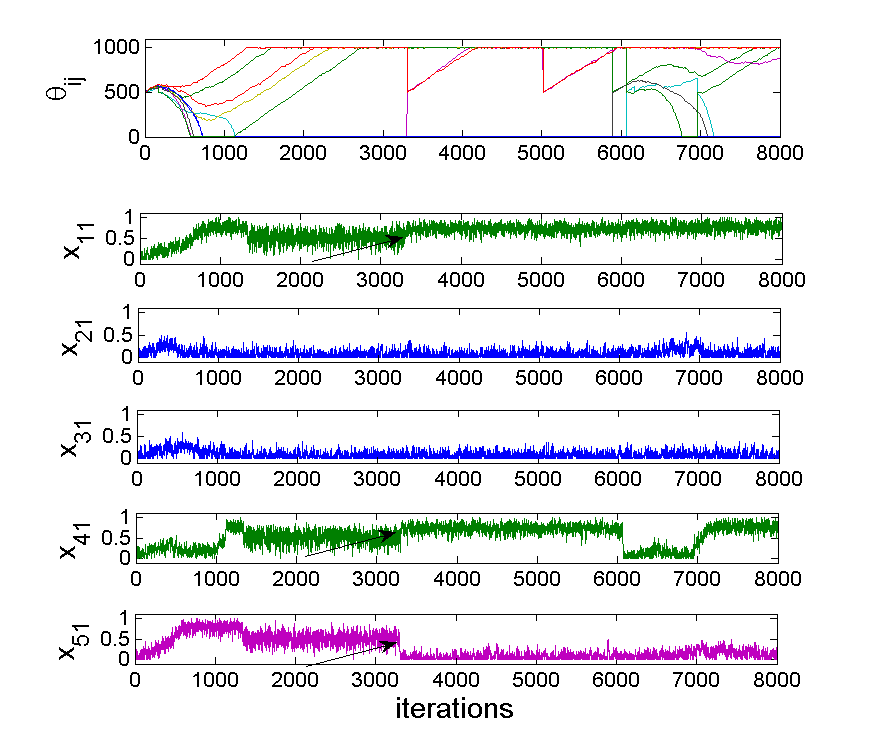
\includegraphics[scale=0.6]{figures/Figure2}\caption{Reinitializing a bee working on a task fulfilled by two other bees after 3250 iterations.}
\label{fig:figure2}
\end{figure}

\par\end{center}

Let us look at the changes in stimuli caused by these two disturbances. In Fig.\ref{fig:figure3}, we observe that there is an immediate recovery because the two other bees instantaneously step up the stimulus does not behave the same way as prior to the disturbance.
In fact, Fig.\ref{fig:figure4} confirms that the mean and the variance of the concerned stimulus increase significantly. One of the reasons behind this change is that the fulfillment of a single job by three different bees is much more stable than when it is performed by only two bees. In the other case we can observe a longer recovery time, after this the concerned stimulus goes back to its initial state; therefore no increase in variance or in mean is perceived. Furthermore, one can notice that the recovery time is bigger than the time that was needed at first by the model to reach its initial equilibrium. This approach of the recovery time will be investigated more deeply in the next section.

\begin{figure}[ht!]
\begin{centering}
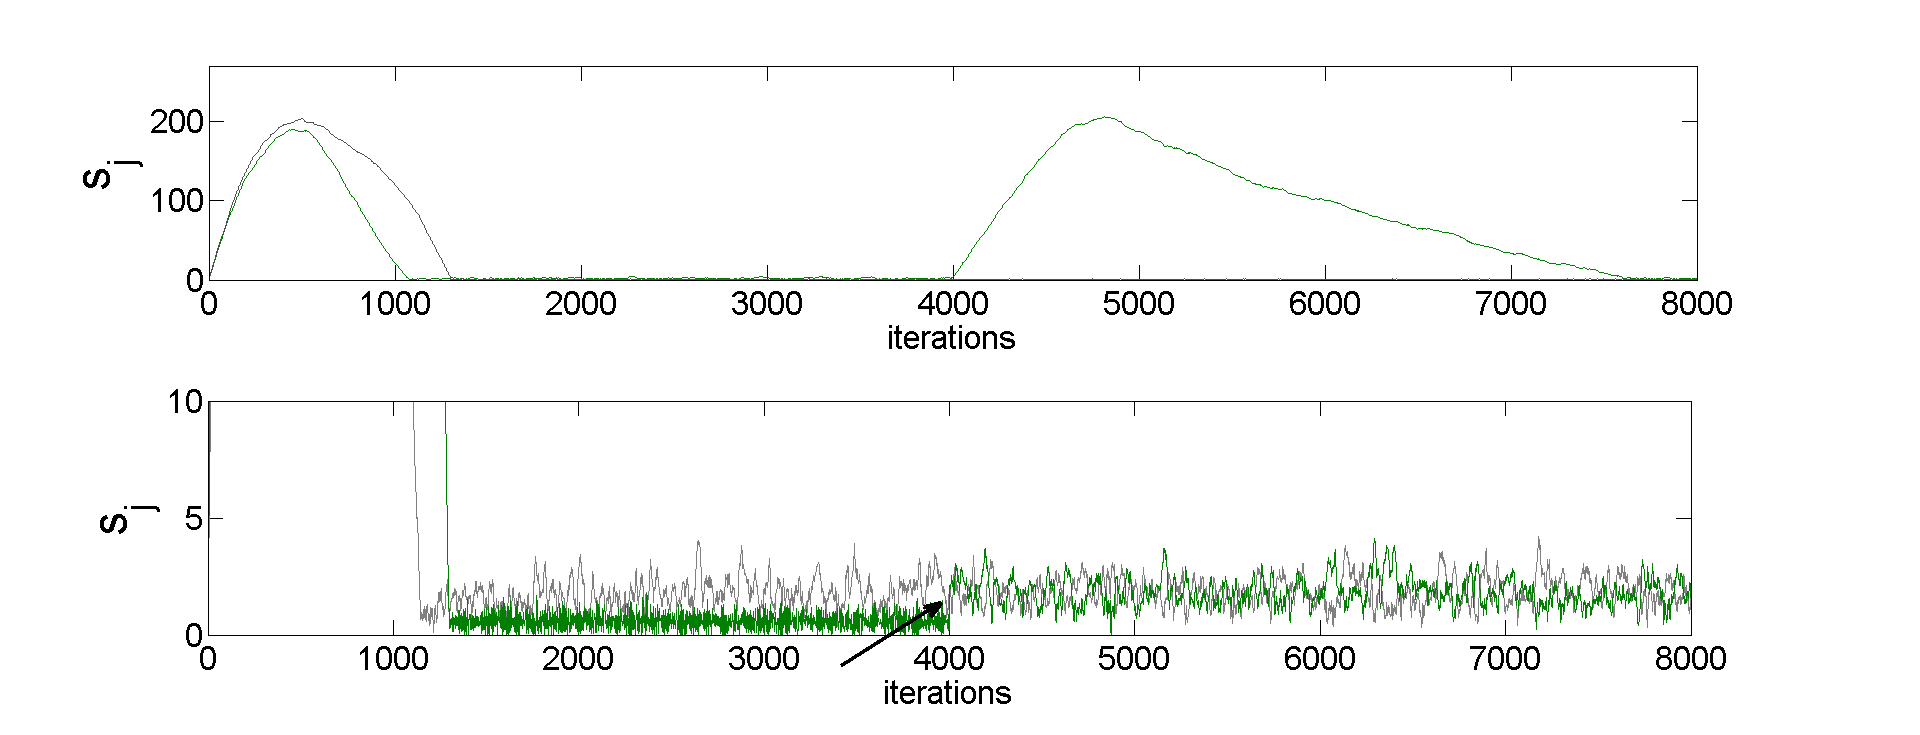
\includegraphics[scale=0.4]{figures/Figure7}\caption{Impact of disturbance on stimulus.}
\label{fig:figure3}
\par\end{centering}

\centering{}
\end{figure}


\begin{figure}[ht!]
\begin{centering}
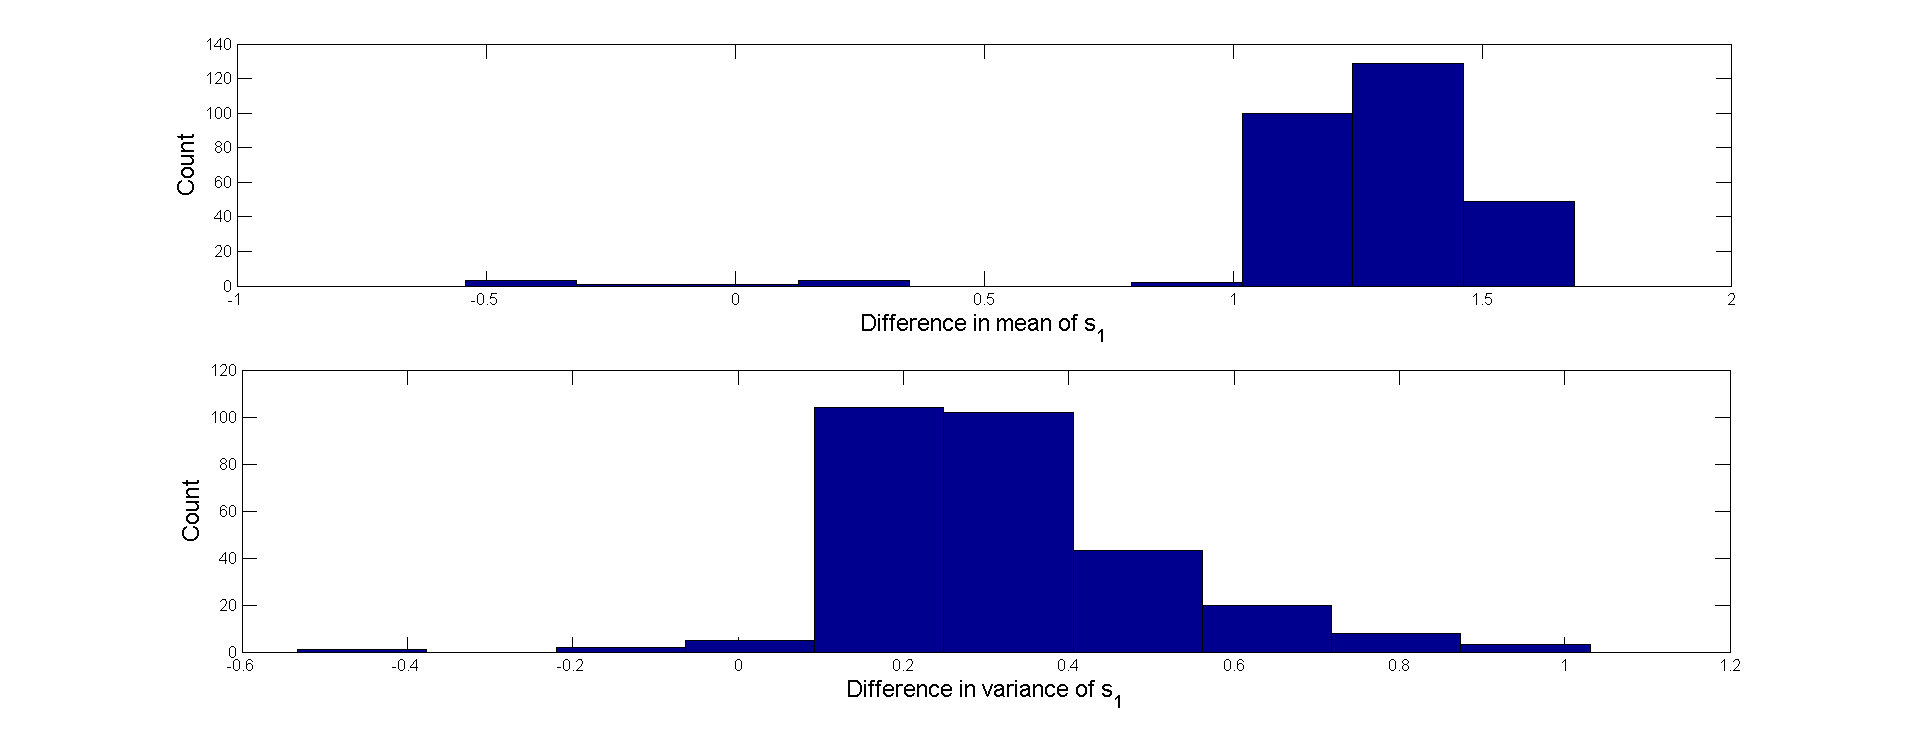
\includegraphics[scale=0.35]{figures/Augmentation2_2}
\label{fig:figure4}
\par\end{centering}

\begin{centering}
\caption{Augmentation of mean and variance of the stimulus after reinitializing a bee working on a task performed by two other bees. \\\hspace{\textwidth} The plot represents a superposition of 500 consecutive runs.}

\par\end{centering}

\end{figure}



\paragraph{Recovery time}


\begin{center}
\begin{figure}[ht!]
\begin{centering}
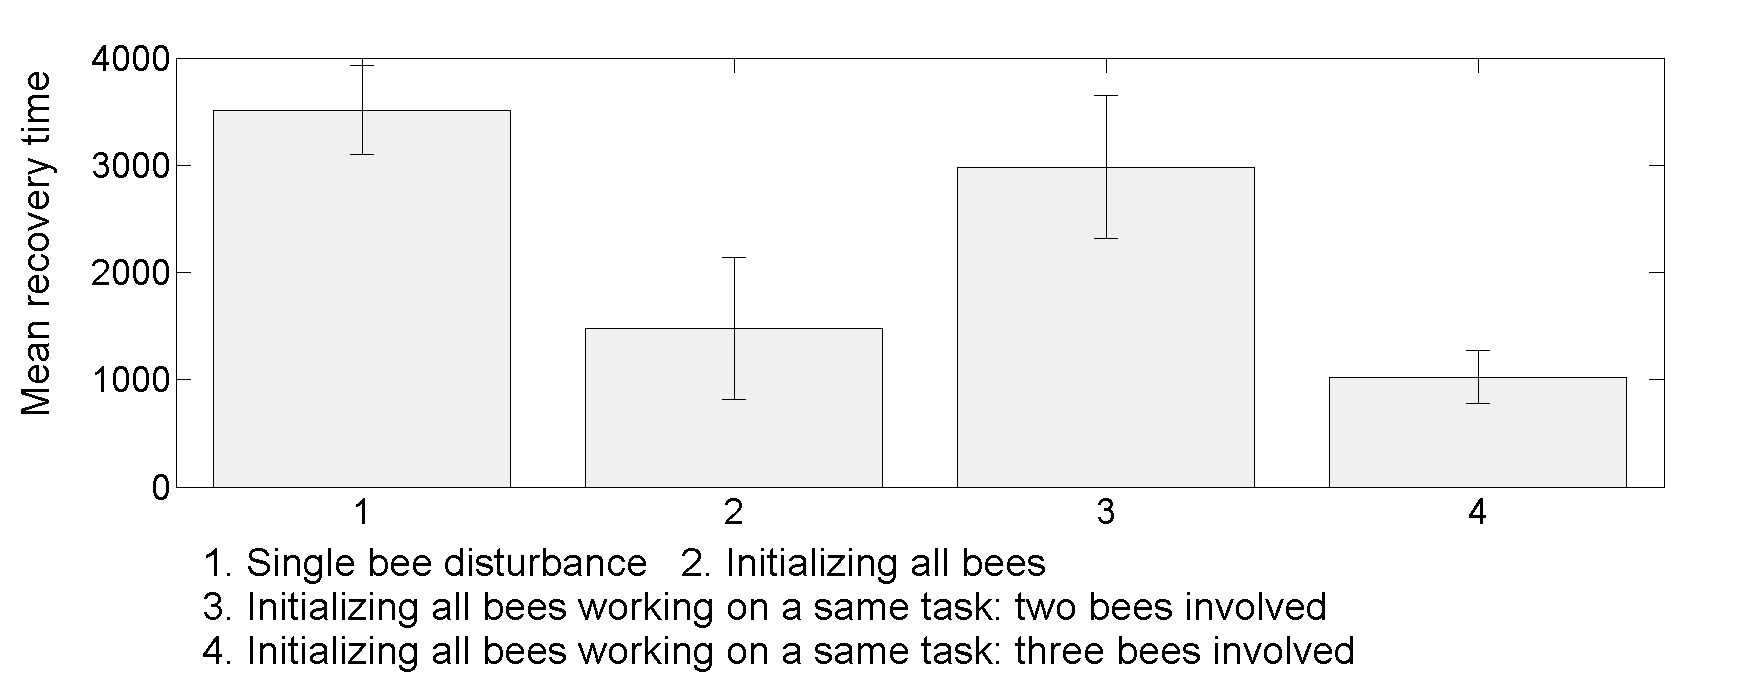
\includegraphics[scale=0.35]{figures/Figure3}
\label{fig:figure5}
\par\end{centering}

\caption{Mean recovery time and associated standard deviation for diverse disturbances. \\\hspace{\textwidth}  Based on 100-200 runs.}


\end{figure}

\par\end{center}

A straightforward measure for the intensity of a disturbance could
be to consider the time of instability generated by this event, or
- in the terms of our model - the time needed to reach low stimuli
again. For this purpose, many simulations have been run to estimate
the average recovery time for various disturbances. Four different
cases have been explored:

First, a single bee is reset, as seen in the previous section; note
that only runs where the bee used to work on a task fulfilled by a
single other bee have been considered, since for the other case the
recovery is immediate. Second, every bee is reinitialized. As it can
be observed in Fig.\ref{fig:figure5}, the recovery time is less significant
in this second case, since the stimuli are more important; the increasing
of the stimuli can be explained because no bee is active. Finally,
every bee working on the same task, for example task 1, are reinitialized.
In this case we need to split the runs: the group of workers performing
the task can be made of two or three bees. In this last case the results
are surprising: the recovery time is way shorter for the group of
three bees than for the one of only two. This could be once again
the cause of a more important peek in stimulus, since more bees are
concerned. This simple argument about the number of bees involved
is not valid if we compare case 2 and case 4, since the number of
tasks concerned is not the same for the two cases. So, as a rule of
thumb, we can say that, on the one hand, for a given number of tasks
(being concerned by the reinitialization) a greater number of bees
involved implies a faster recovery and, on the other hand, for a given
number of bees, a greater number of tasks implies a slower recovery.

Therefore, this method is a good way to quantify the intensity of
some disturbance. However this approach is limited to simple cases
where recovery can be observed.

\subsection{Dynamical Population within the Theraulaz Model}

The assumption that the colony size does not evolve in time is an
important simplification of the reality. Therefore, we have attempted
to extend the previous model to a more dynamical one. 


\subsubsection{Model Extension}

The crutial extension is that N(t) is now depending on time. This
is a fundamental change in the model and it raises many new implementation
problems. First, the size of the vector that is processed by the ordinary
differential equation solver changes frequently; to solve this problem
a more dynamical solver is required. Second, the number of bees is
one of the predominant factors influencing the computational intensity
of the simulation; N should therefore reach some sort of dynamical
equilibrium or stay into a given range. And finally it is more complicated
to keep the full history of the variables.

About the extension, on one hand, a probability of birth of a new
bee is introduced which is linearly dependent to the welfare of the
society. This seems to be a natural choice, since the welfare was
defined as the ability of the society to fulfill all its needs. On
the other hand, a probability of death was also introduced which is
inversely proportional to the welfare of the society. This stochastic
approach allows to get a more realistic model, since birth can occur
even in difficult moments. Those are the main changes, the other ones
are mainly technical and we'll not be presented.


\subsubsection{First results}

Before considering the result of the extend model, we'll have a look
at some simple cases

First, we can observe in Fig.\ref{fig:figure6} that killing a bee that used
to work on a task performed by only one other bee, implies a change
of specialization for one of the remaining bee, since the task is
now highly undersupplied. We can also notice that the two bees that
do not make the effort to swtich their task, work harder to compensate
the loss implied by other bee.

\begin{figure}
\begin{centering}
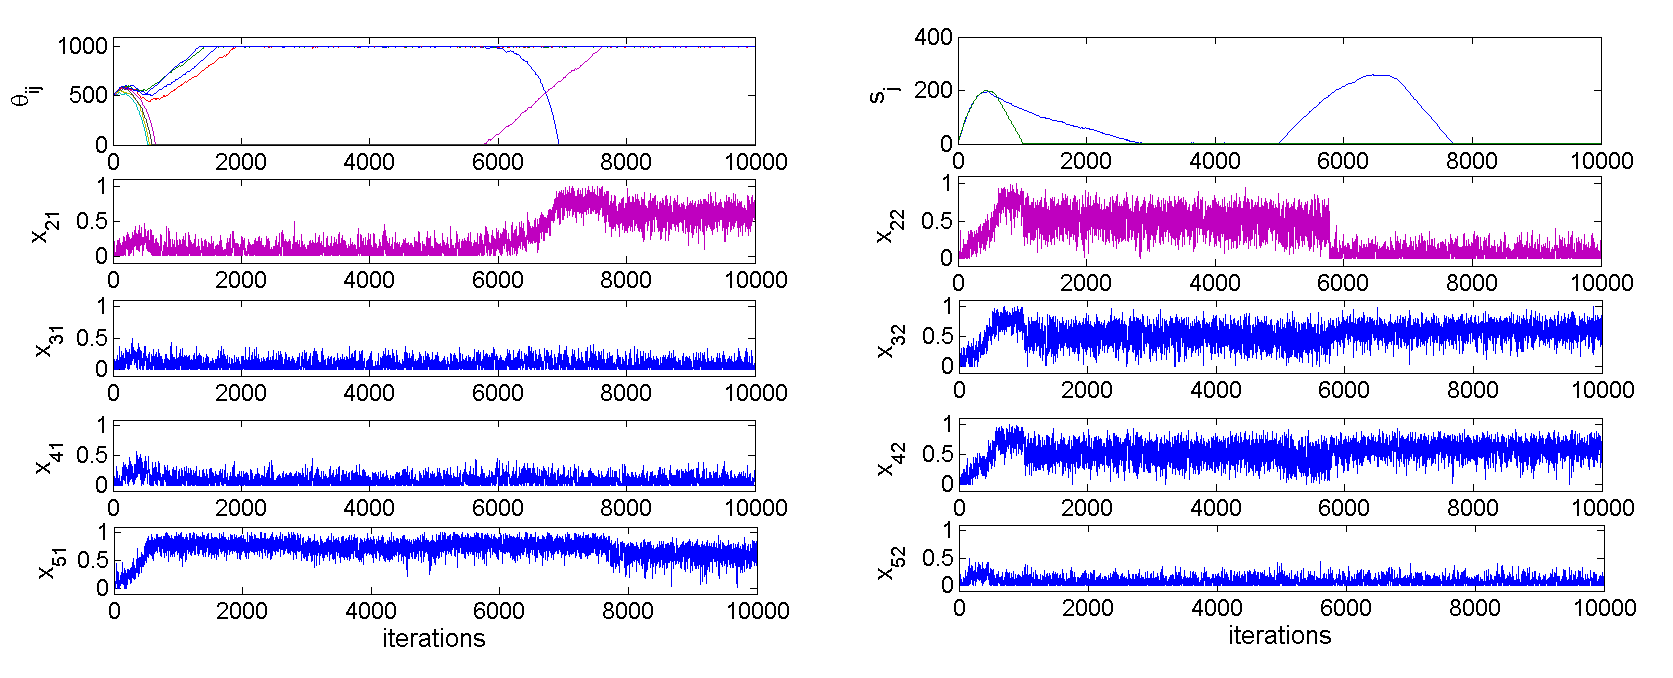
\includegraphics[scale=0.4]{figures/Figure4}
\label{fig:figure6}
\par\end{centering}

\centering{}\caption{Reorganization of the colony after the death of a bee after 5000 iterations}
\end{figure}


Second, we can observe in Fig.\ref{fig:figure7} that introducing two new bees
simultaneously increases the stimuli, since those bees choose not
to work at first. One of the reasons behind this inactivity is the
fact that the stimuli are still small when they come into the society.
However, at a certain time the stimulus is so high that the bees decide
to work and after a few iterations an equilibrium is reached.

\begin{figure}[ht!]
\begin{centering}
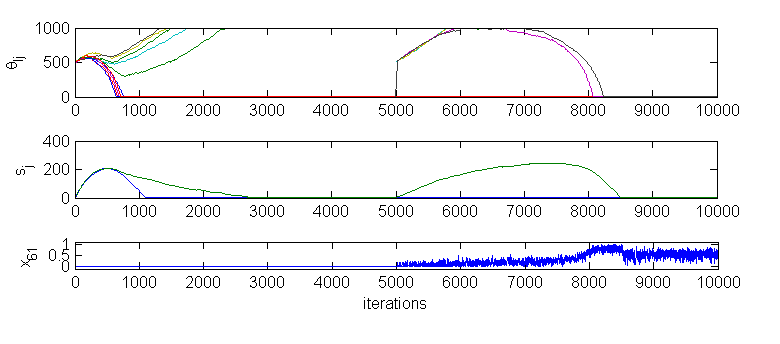
\includegraphics[scale=0.8]{figures/Figure5}
\label{fig:figure7}
\par\end{centering}

\centering{}\caption{Introduction of two new bees in the society after 5000 iterations}
\end{figure}


We can notice with those two examples, that birth or death of a bee
often disturbed the state the society. Here, the effects are amplified
because of the small size of the society and we'll see in the next
section that larger societies have no problem to incorporate a few
new bees.


\subsubsection{Main result}

After a few runs of our new dynamical model, we can start making a
few observations. The dynamics of the $\theta_{ij}$ are hard to capture,
because of the complexity of the process. However, simple observations
can be made by considering the $s_{j}$ and the N(t) . First, the
number of bees increases drastically at the beginning of the simulation
before reaching an oscillatory state. Second, cycles can be observed
for the wealth. The reason behind this cycling effeft is that when
the welfare is high many new bees are introduced. Such bees have medium
thresholds and low $x_{ij}$ - to many of those is going to increase
the stimulus and the instability of the colony. On the other side,
if the wealth is low the number of bees introduced are low and then
the above mentioned disturbance does not occur.

It is important to notice that the cycles for the stimuli have been
observed for most of the runs, however the nice welfare cycles can
only be observe if the phase difference between the two task is not
to important. 

\begin{figure}[ht!]
\begin{centering}
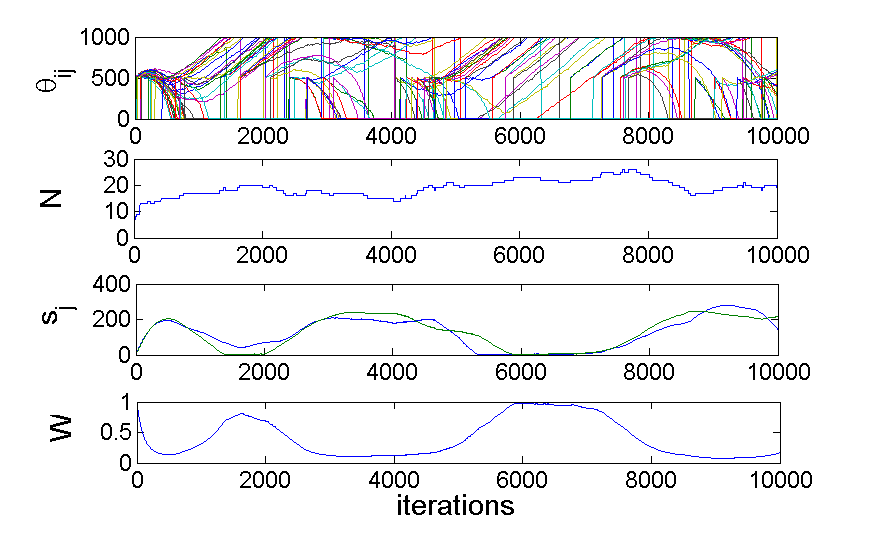
\includegraphics[scale=0.8]{figures/Figure6}
\label{fig:figure8}
\par\end{centering}

\begin{centering}
\caption{Run of the new dynamical model}

\par\end{centering}

\end{figure}




\subsubsection{Comments}

Deeper analysis could be useful to have a more precise idea of the
dynamics behind this model. For example, it would be interesting to
determine the conditions either under which the colony disappears or under
which a dynamical equilibrium can be found. Furthermore, it would
be interesting to test the reactions of the model to a higher number
of tasks. In conclusion, this dynamical evolution of the colony size
opens a wide range of new investigation possibilities and this extension
is a key step towards a more precise and general model.


Deeper analysis could be useful to have a more precise idea of the
dynamics behind this model. For example, it would be interesting to
determine the conditions under which the colony disappears or under
which a dynamical equilibrium can be found. Furthermore, it would
be interesting to test the reactions of the model to a higher number
of tasks. In conclusion, this dynamical evolution of the colony size
opens a wide range of new investigation possibilities and this extension
is a key step towards a more precise and general model.
%\end{document}

 

\subsection{PBM Model}
The PBM model is quite robust and a broad range of parameters deliver sensible results. Below we describe the influence of the more important parameters on time-dependant quantities such as allocated tasks, productivities, boredoms and salaries. 

Parameters for a standard simulation could be the following: $N=7$, $M=3$, $\lambda=0.01$, $\kappa=0.003$, $\zeta=0.001$, $\eta=0.0003$, $p_s=0.003$, $\Delta t=1$, $A_\mu=3$, $A_\sigma=0.7$, $P_\mu=2$, $P_\sigma=0.7$, $B_\mu=0.5$, $B_\sigma=0.15$. Figure~\ref{fig:sim1task} shows the time evolution of the tasks performed by the different workers. It allows to see the dynamics of work allocation. Figures~\ref{fig:sim1prod}, \ref{fig:sim1money} and \ref{fig:sim1boredom} allow to understand the motivation for choosing another task. Figure~\ref{fig:sim1prod} shows the evolution of the productivity at the current tasks and explains why workers performing the same task do not earn the same amount of money, which can be seen in Figure~\ref{fig:sim1money}. Figure~\ref{fig:sim1boredom} displays the evolution of the boredom. It illustrates that a too high boredom can induce a change of task even if the new task is less paid than the previous one. A general observation is that people working on tasks at which their maximam boredom is high tend to change the task rapidly because of the rapid increase of the boredom. Figure~\ref{fig:sim1totalmoney} shows the total amount of money earned so far by each of the workers. It features a pronounced social inequality, which is caused by two main factors. Firstly, the inherent characteristics of the workers make some of them much more productive, thence earning more money. The second factor has its origin in the society, more precisely in the production of other individuals; it could be illustrated by the fact that a not particularly skilled individual will be remunerated a lot if he is the only one able to do his job, while two very skilled individuals at the same task will earn much less.

\begin{figure}[hp!]
	\centering
	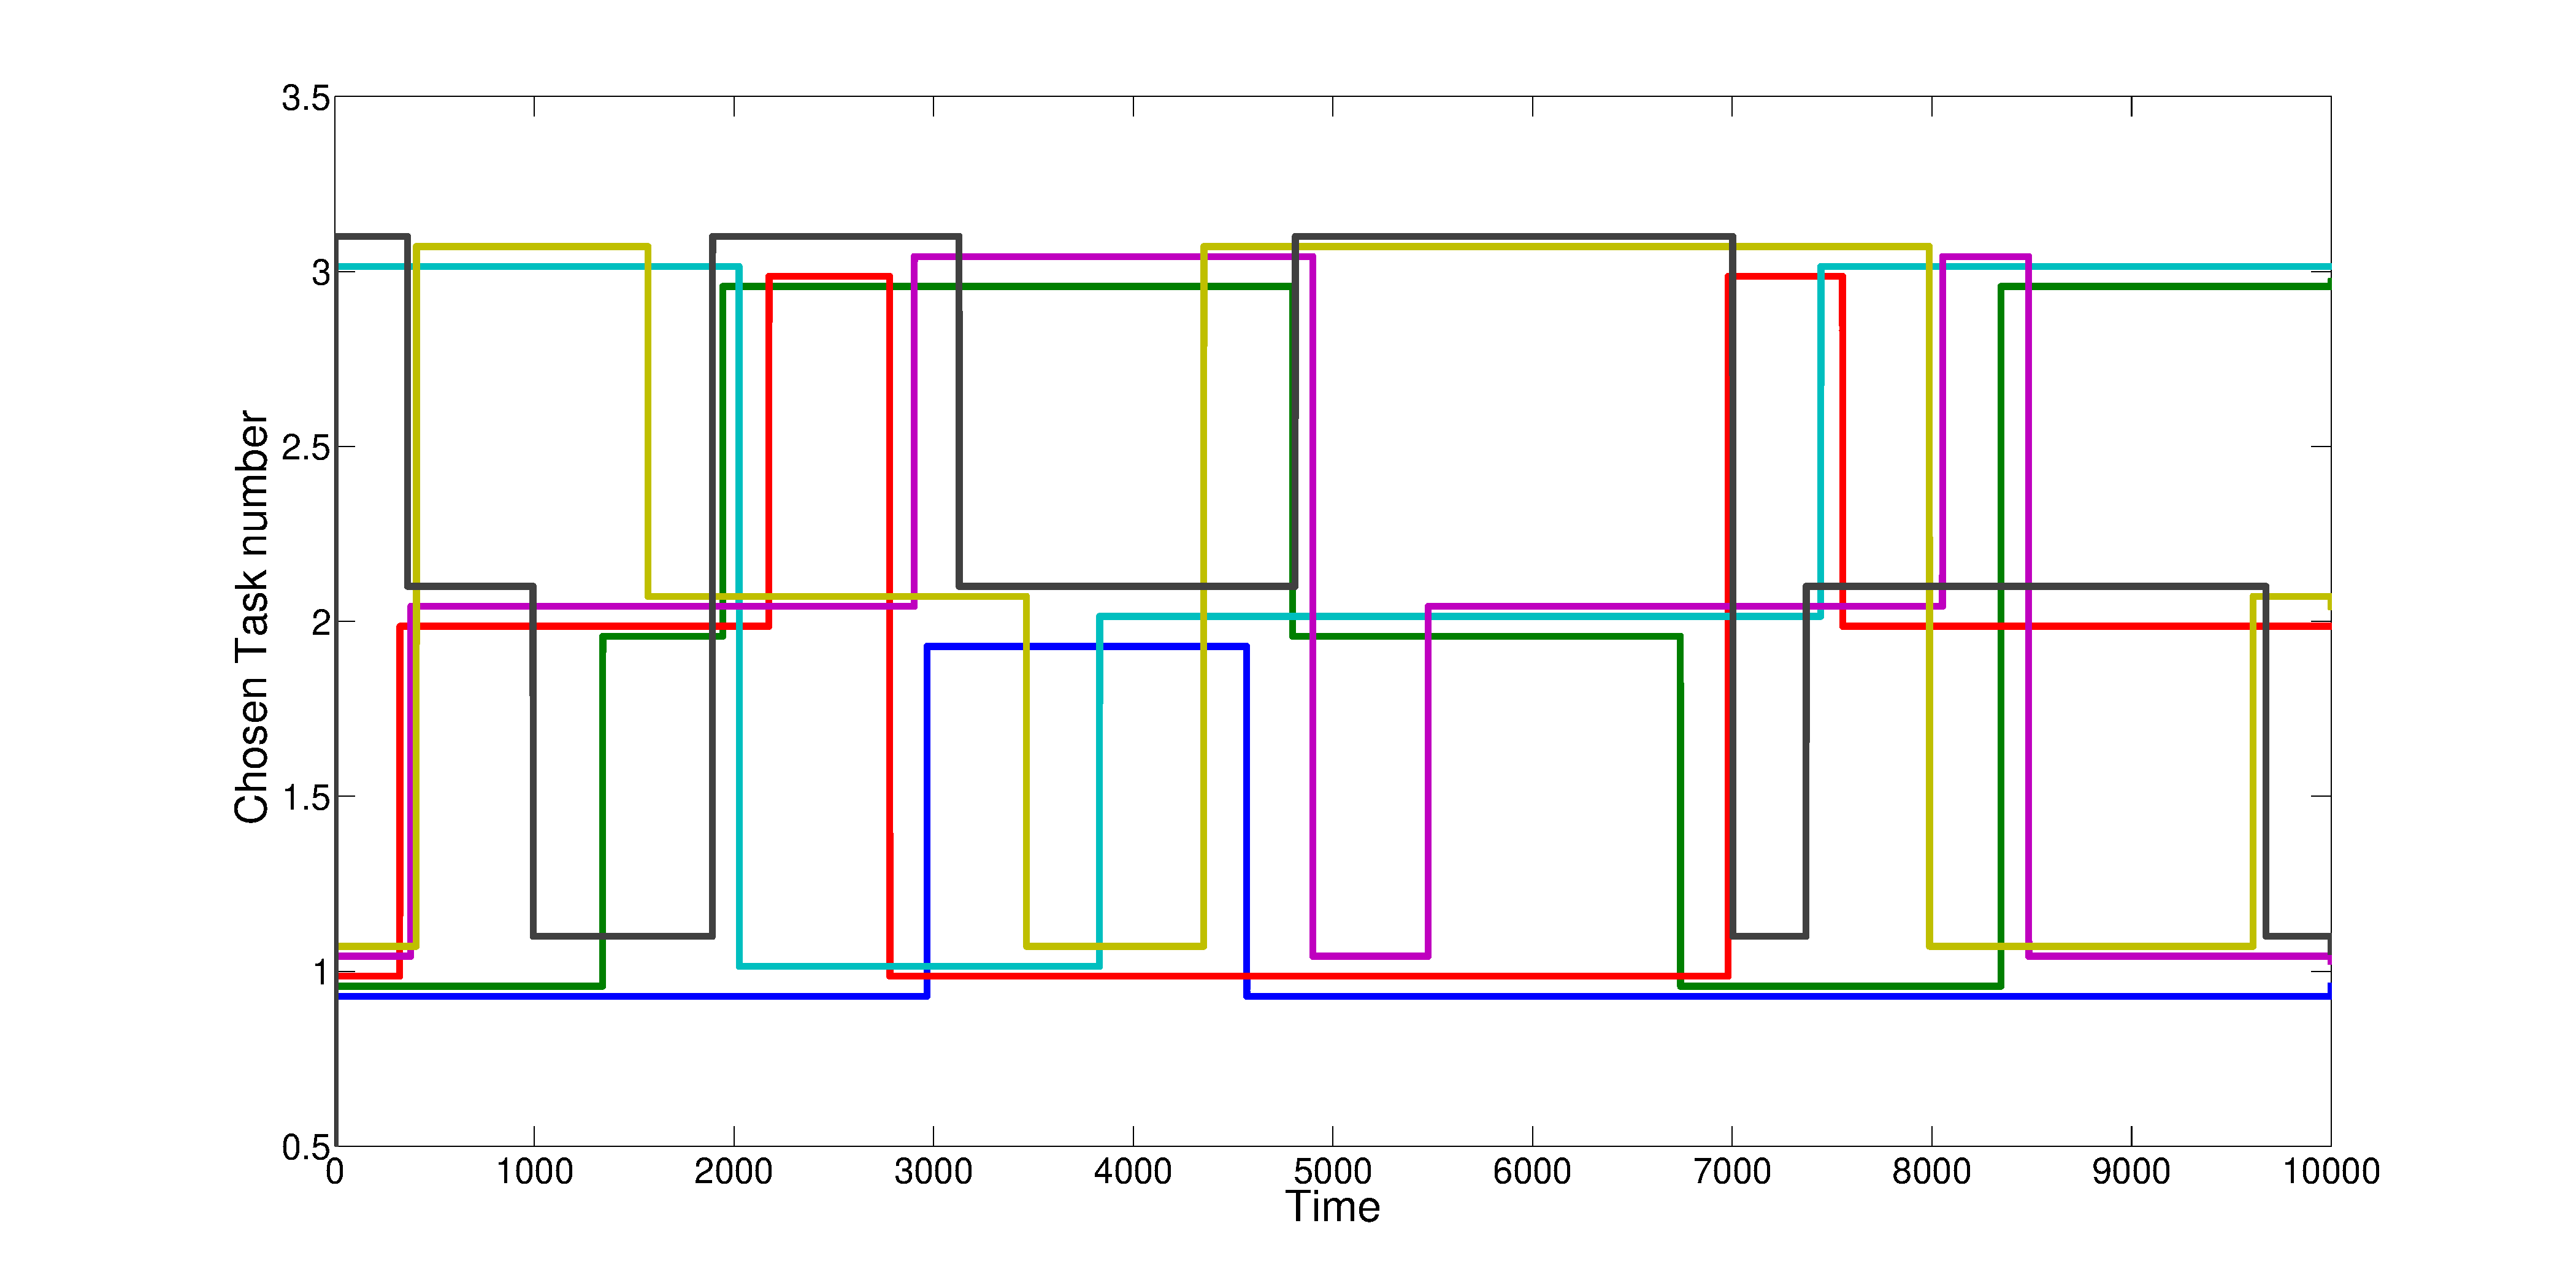
\includegraphics[width=0.9\textwidth]{figures/taskno.pdf}
	\caption{Current tasks of the workers as a function of time. Each worker is represented by a different color. The curves of the different individui have a small vertical shift so that all the lines are visible.}
	\label{fig:sim1task}
\end{figure}

\begin{figure}[hp!]
	\centering
	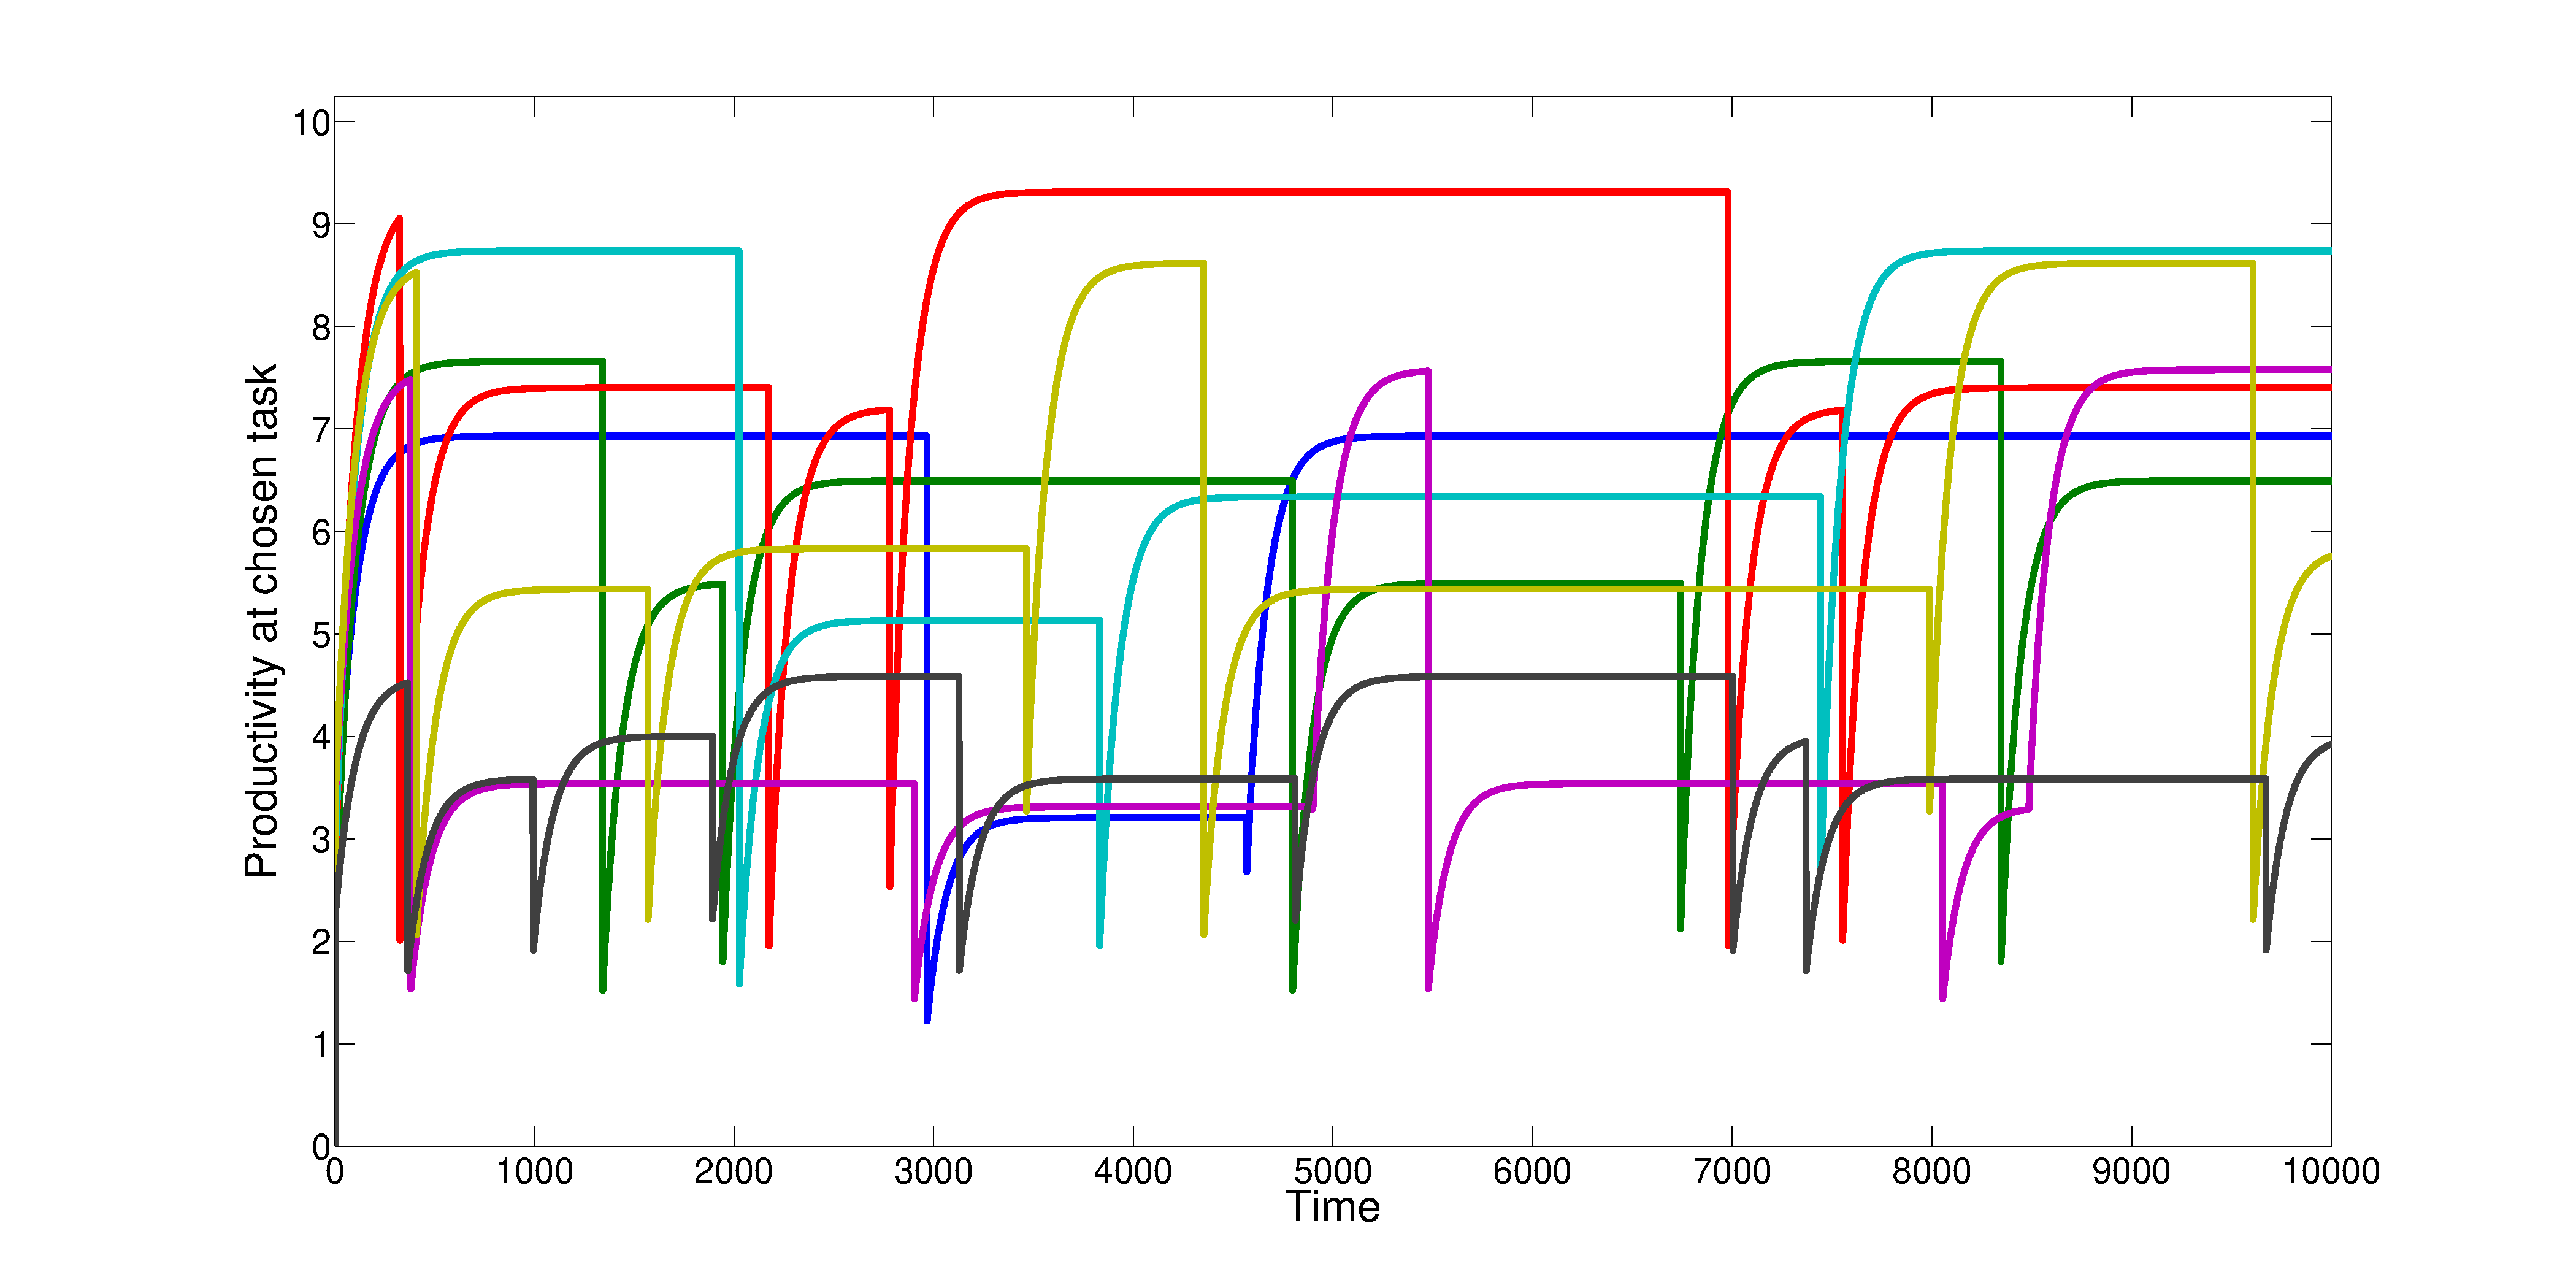
\includegraphics[width=0.9\textwidth]{figures/productivity.pdf}
	\caption{Productivity of the workers at the tasks they are currently performing. The incontinuities mark a change in the task and correspond to what is shown in Figure~\ref{fig:sim1task}.}
	\label{fig:sim1prod}
\end{figure}

\begin{figure}[hp!]
	\centering
	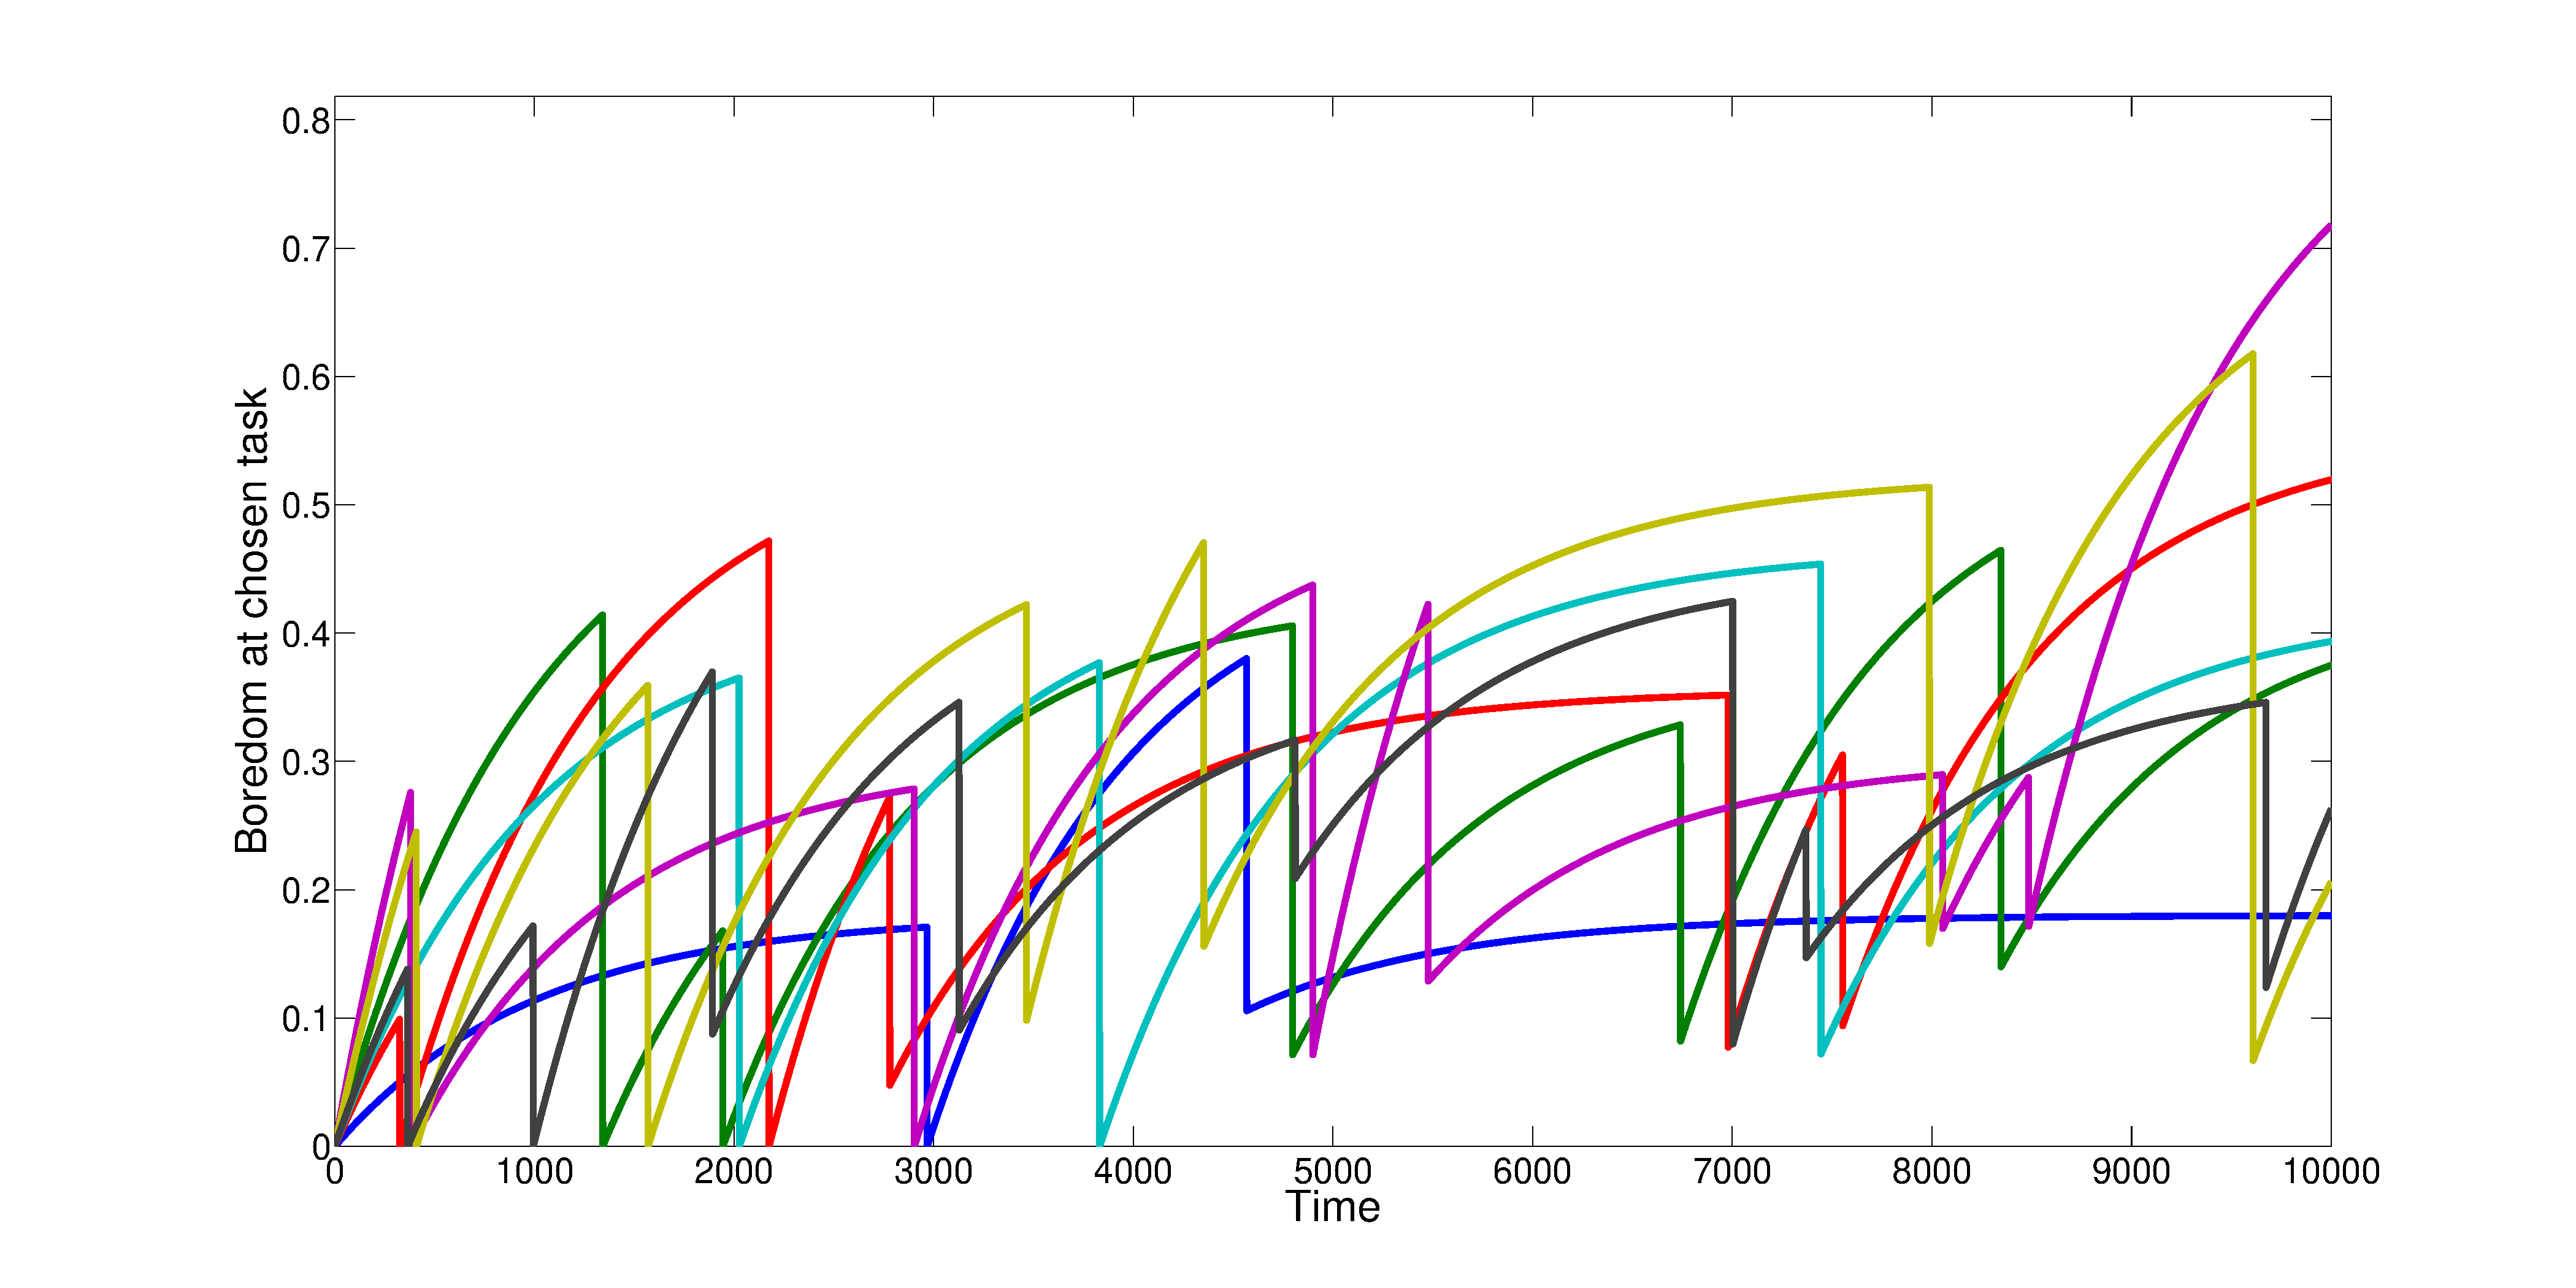
\includegraphics[width=0.9\textwidth]{figures/boredom.pdf}
	\caption{Boredom of the workers at the tasks they are currently performing. It can be seen that the maximal boredom is not achieved in most of the cases, since the boredom becomes too high.}
	\label{fig:sim1boredom}
\end{figure}

\begin{figure}[hp!]
	\centering
	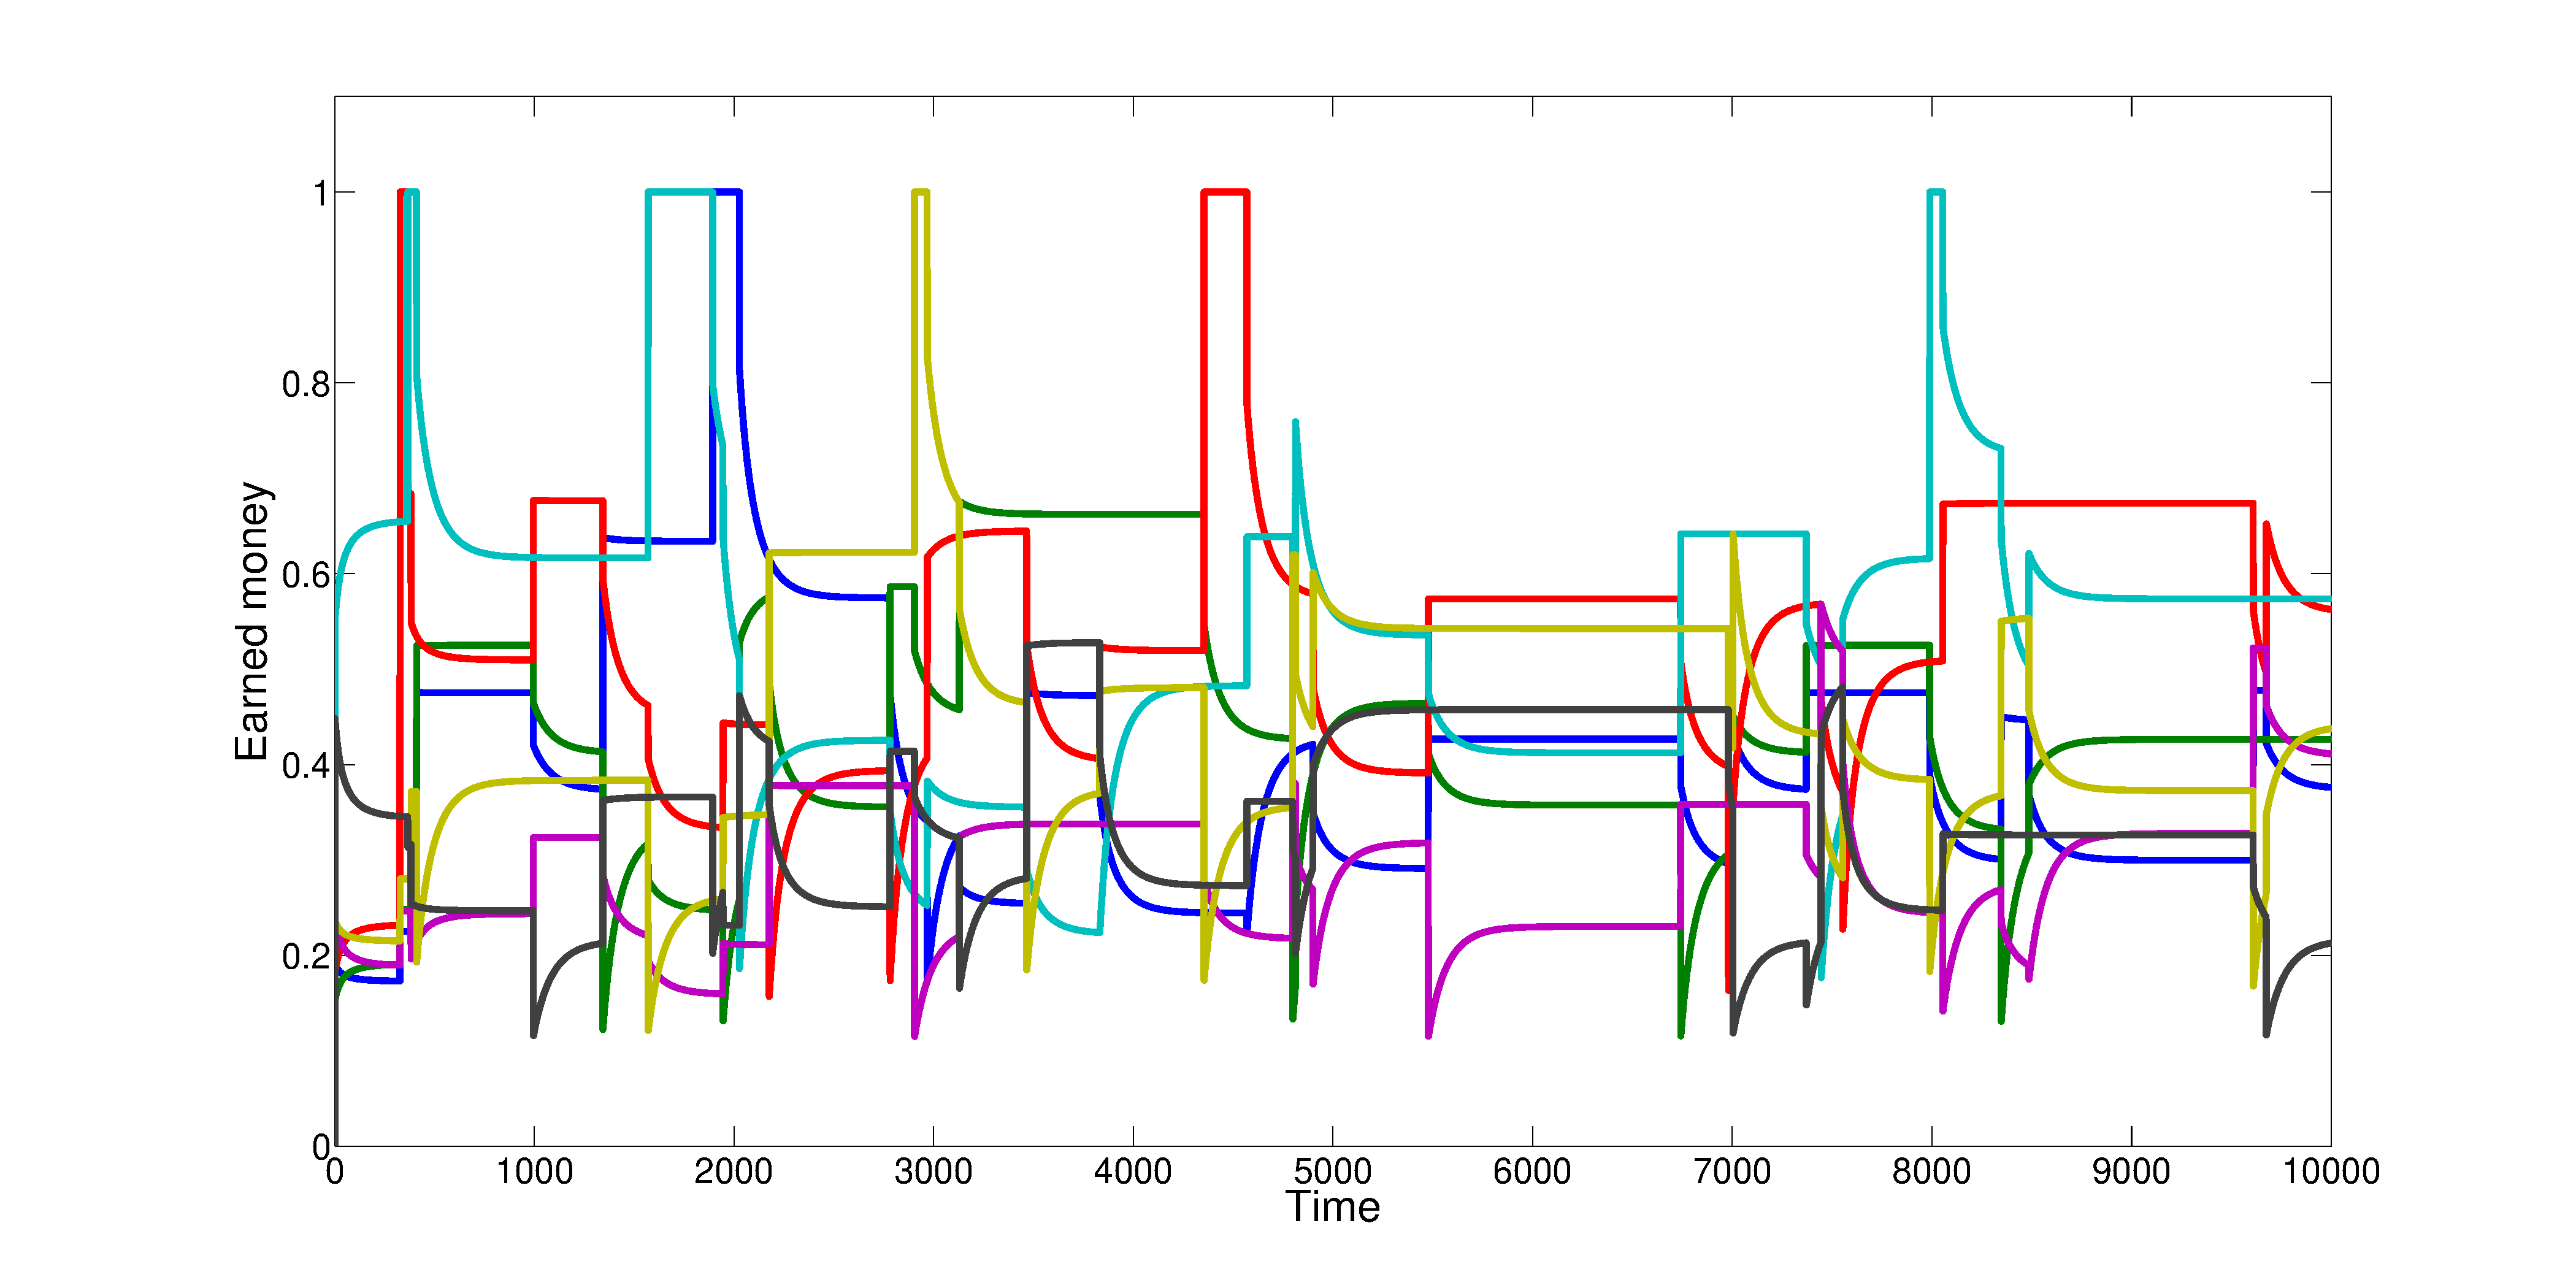
\includegraphics[width=0.9\textwidth]{figures/money.pdf}
	\caption{Salary of the workers as a function of time. A salary of 1 means that a worker is the only one to perform his current task and therefore gets all the money granted to the task.}
	\label{fig:sim1money}
\end{figure}

\begin{figure}[hp!]
	\centering
	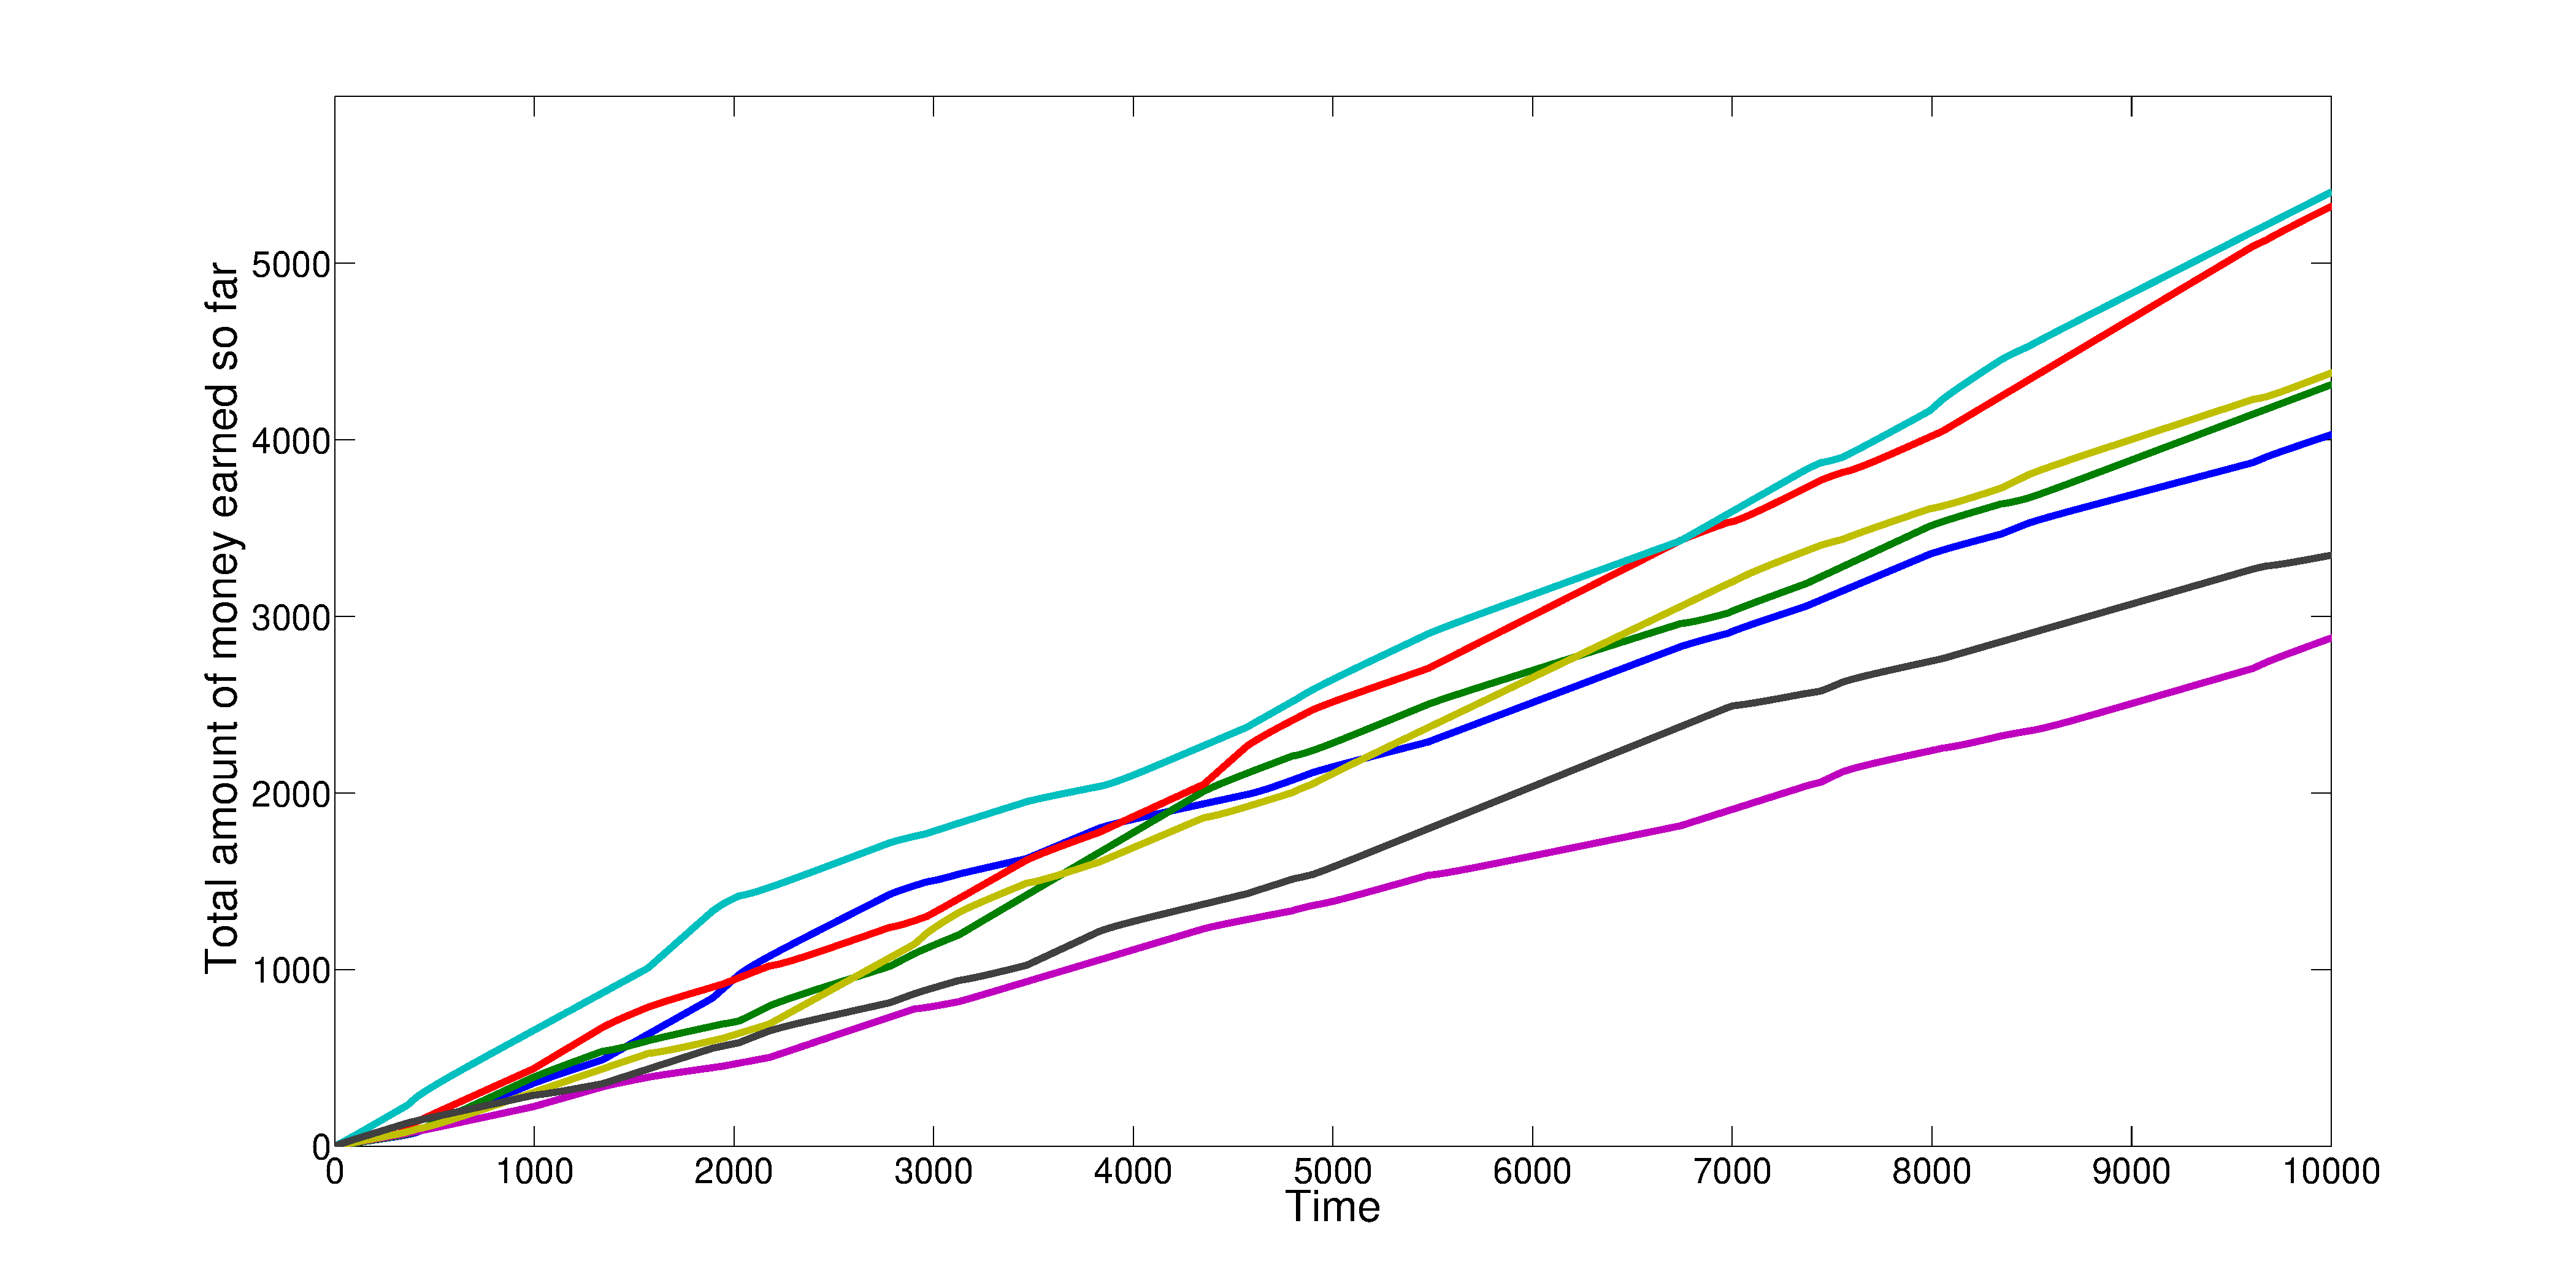
\includegraphics[width=0.9\textwidth]{figures/totalmoney.pdf}
	\caption{Total money earned by each of the workers. It illustrates how the social inequalities are steadily increasing, and the hierarchy of the society stays the same over during the simulation.}
	\label{fig:sim1totalmoney}
\end{figure}

The randomness used in generation of the productivities $P_{ij}$ and of the abilities $A_i$ allow the inspection of social inequality. Both quantities have a similar influence, with the difference that the differences in $P_{ij}$ are both task- and worker-specific, while the differences in $A_i$ are worker-specific. Setting the standard deviation of the distributions to zero would result in a model with much less social inequality, which is not the scope of the present model. The larger the standard deviation, the more pronounced the social inequalities will be. Figures~\ref{fig:sd1} and \ref{fig:sd2} illustrate the influence of the standard deviation used for the generation of the abilities and the initial productivities on social inequality.

\begin{figure}[hp!]
	\centering
	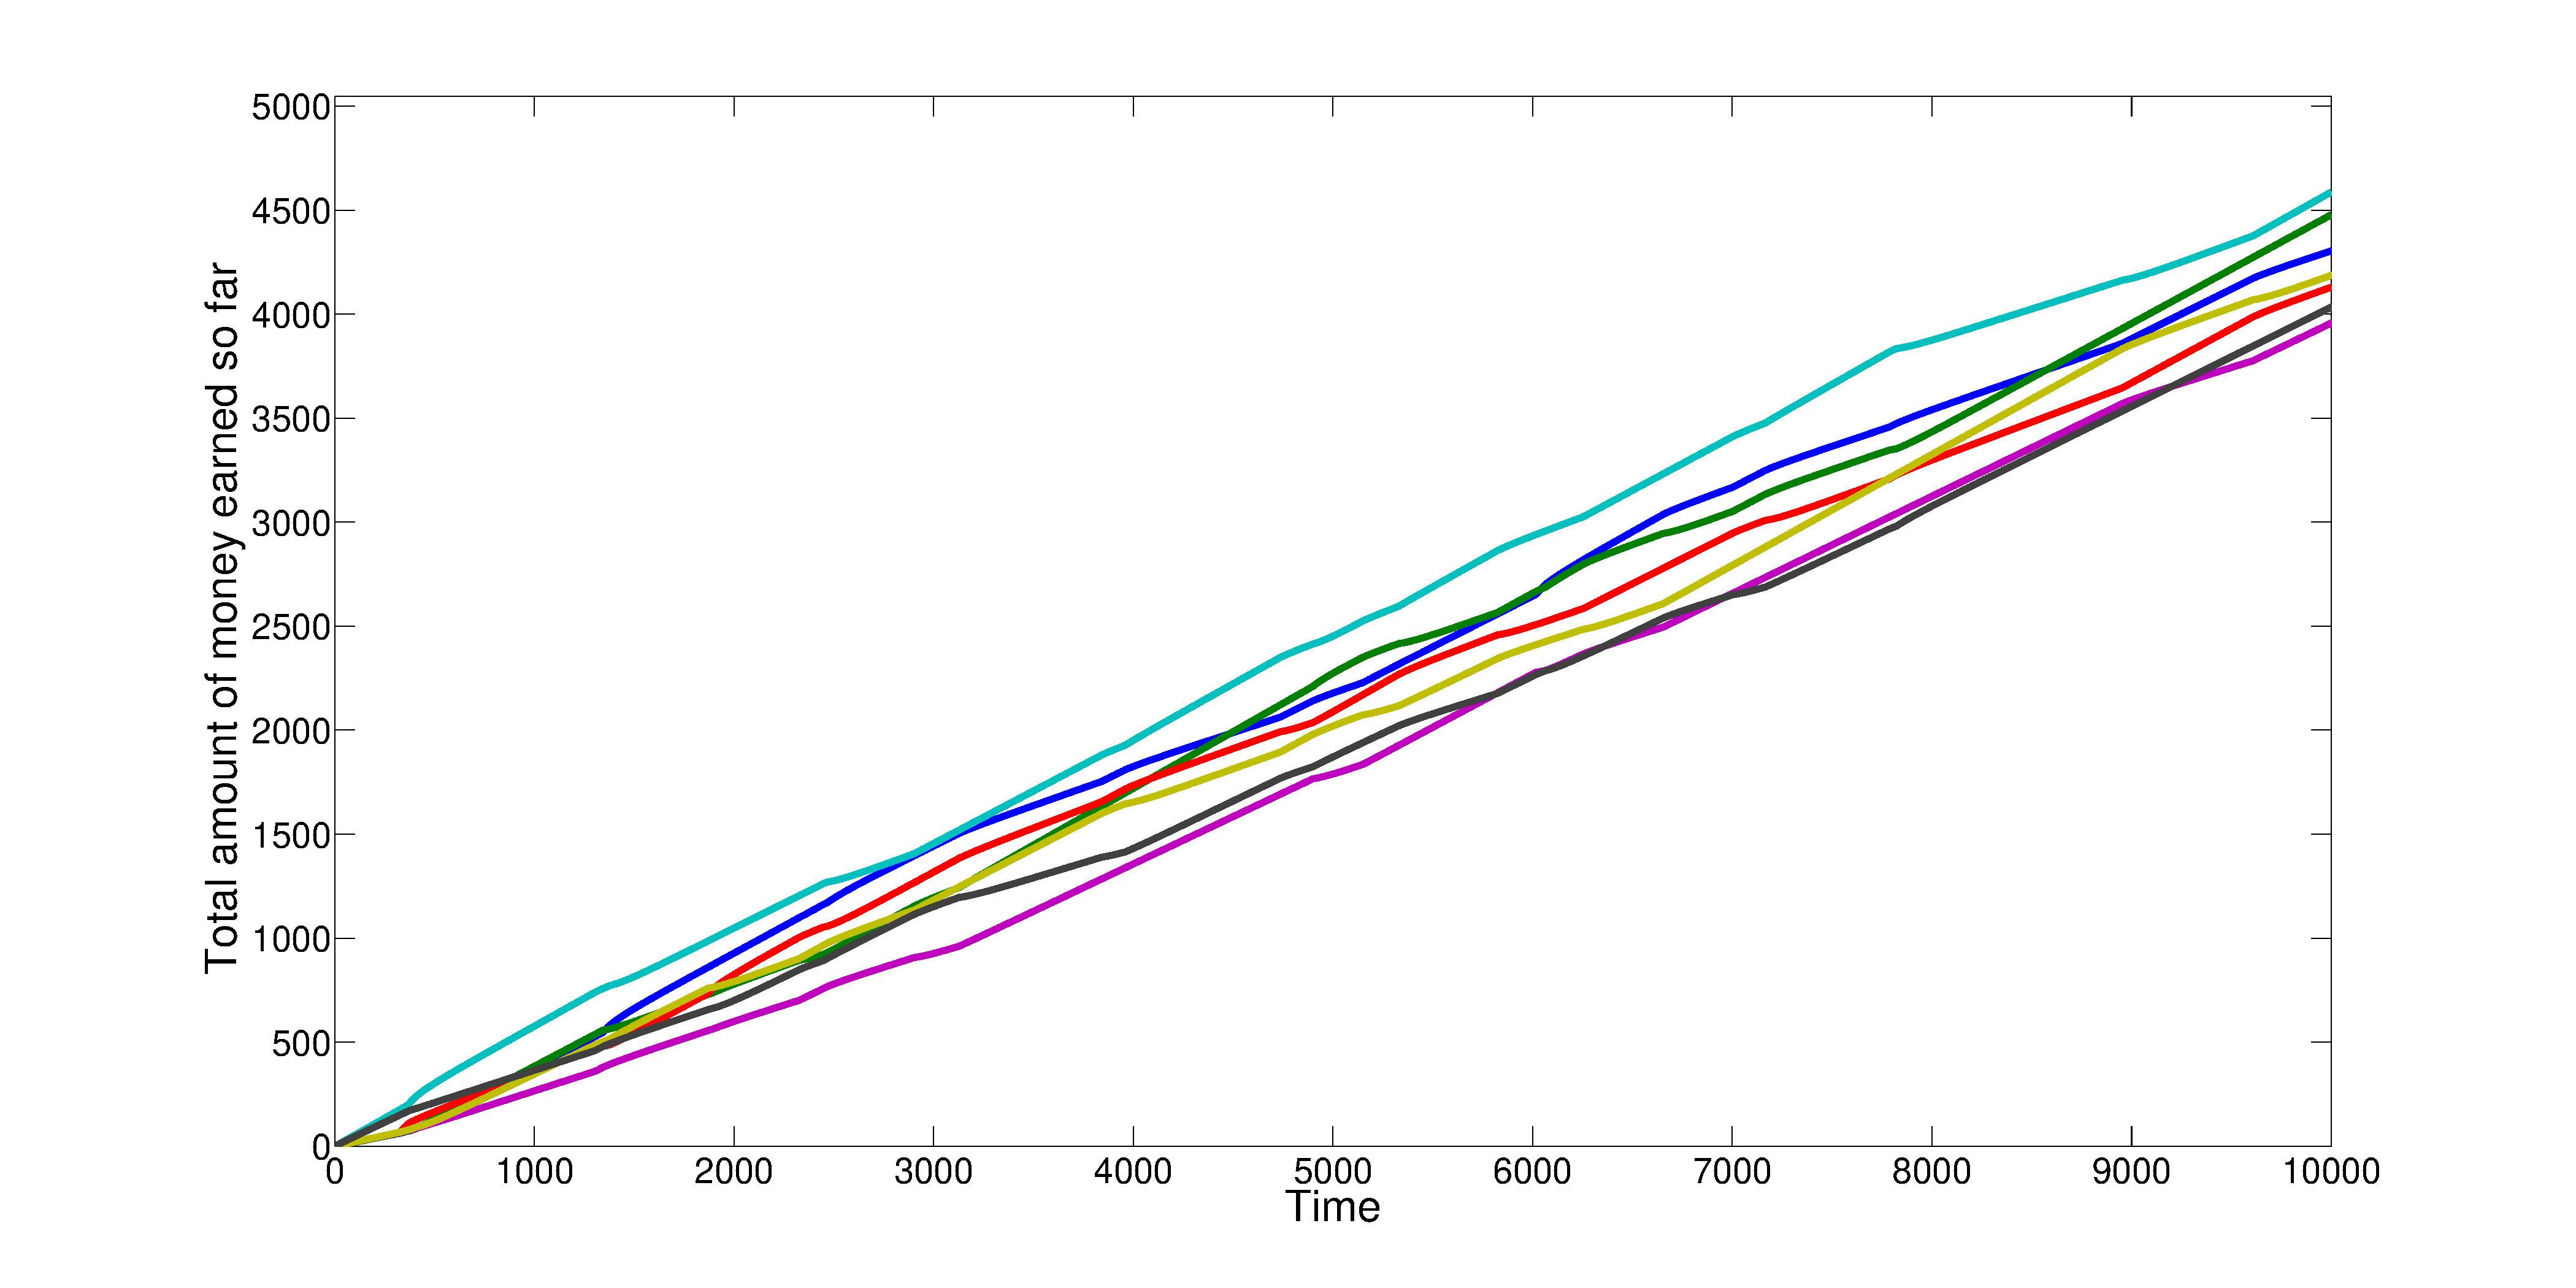
\includegraphics[width=0.9\textwidth]{figures/sd1.pdf}
	\caption{Total money earned by each of the workers. But for $P_\sigma=0.2$ and $A_\sigma=0.2$, the same parameters as in Figure~\ref{fig:sim1totalmoney} were used. The social inequalities remain narrow and do not increase a lot with time.}
	\label{fig:sd1}
\end{figure}

\begin{figure}[hp!]
	\centering
	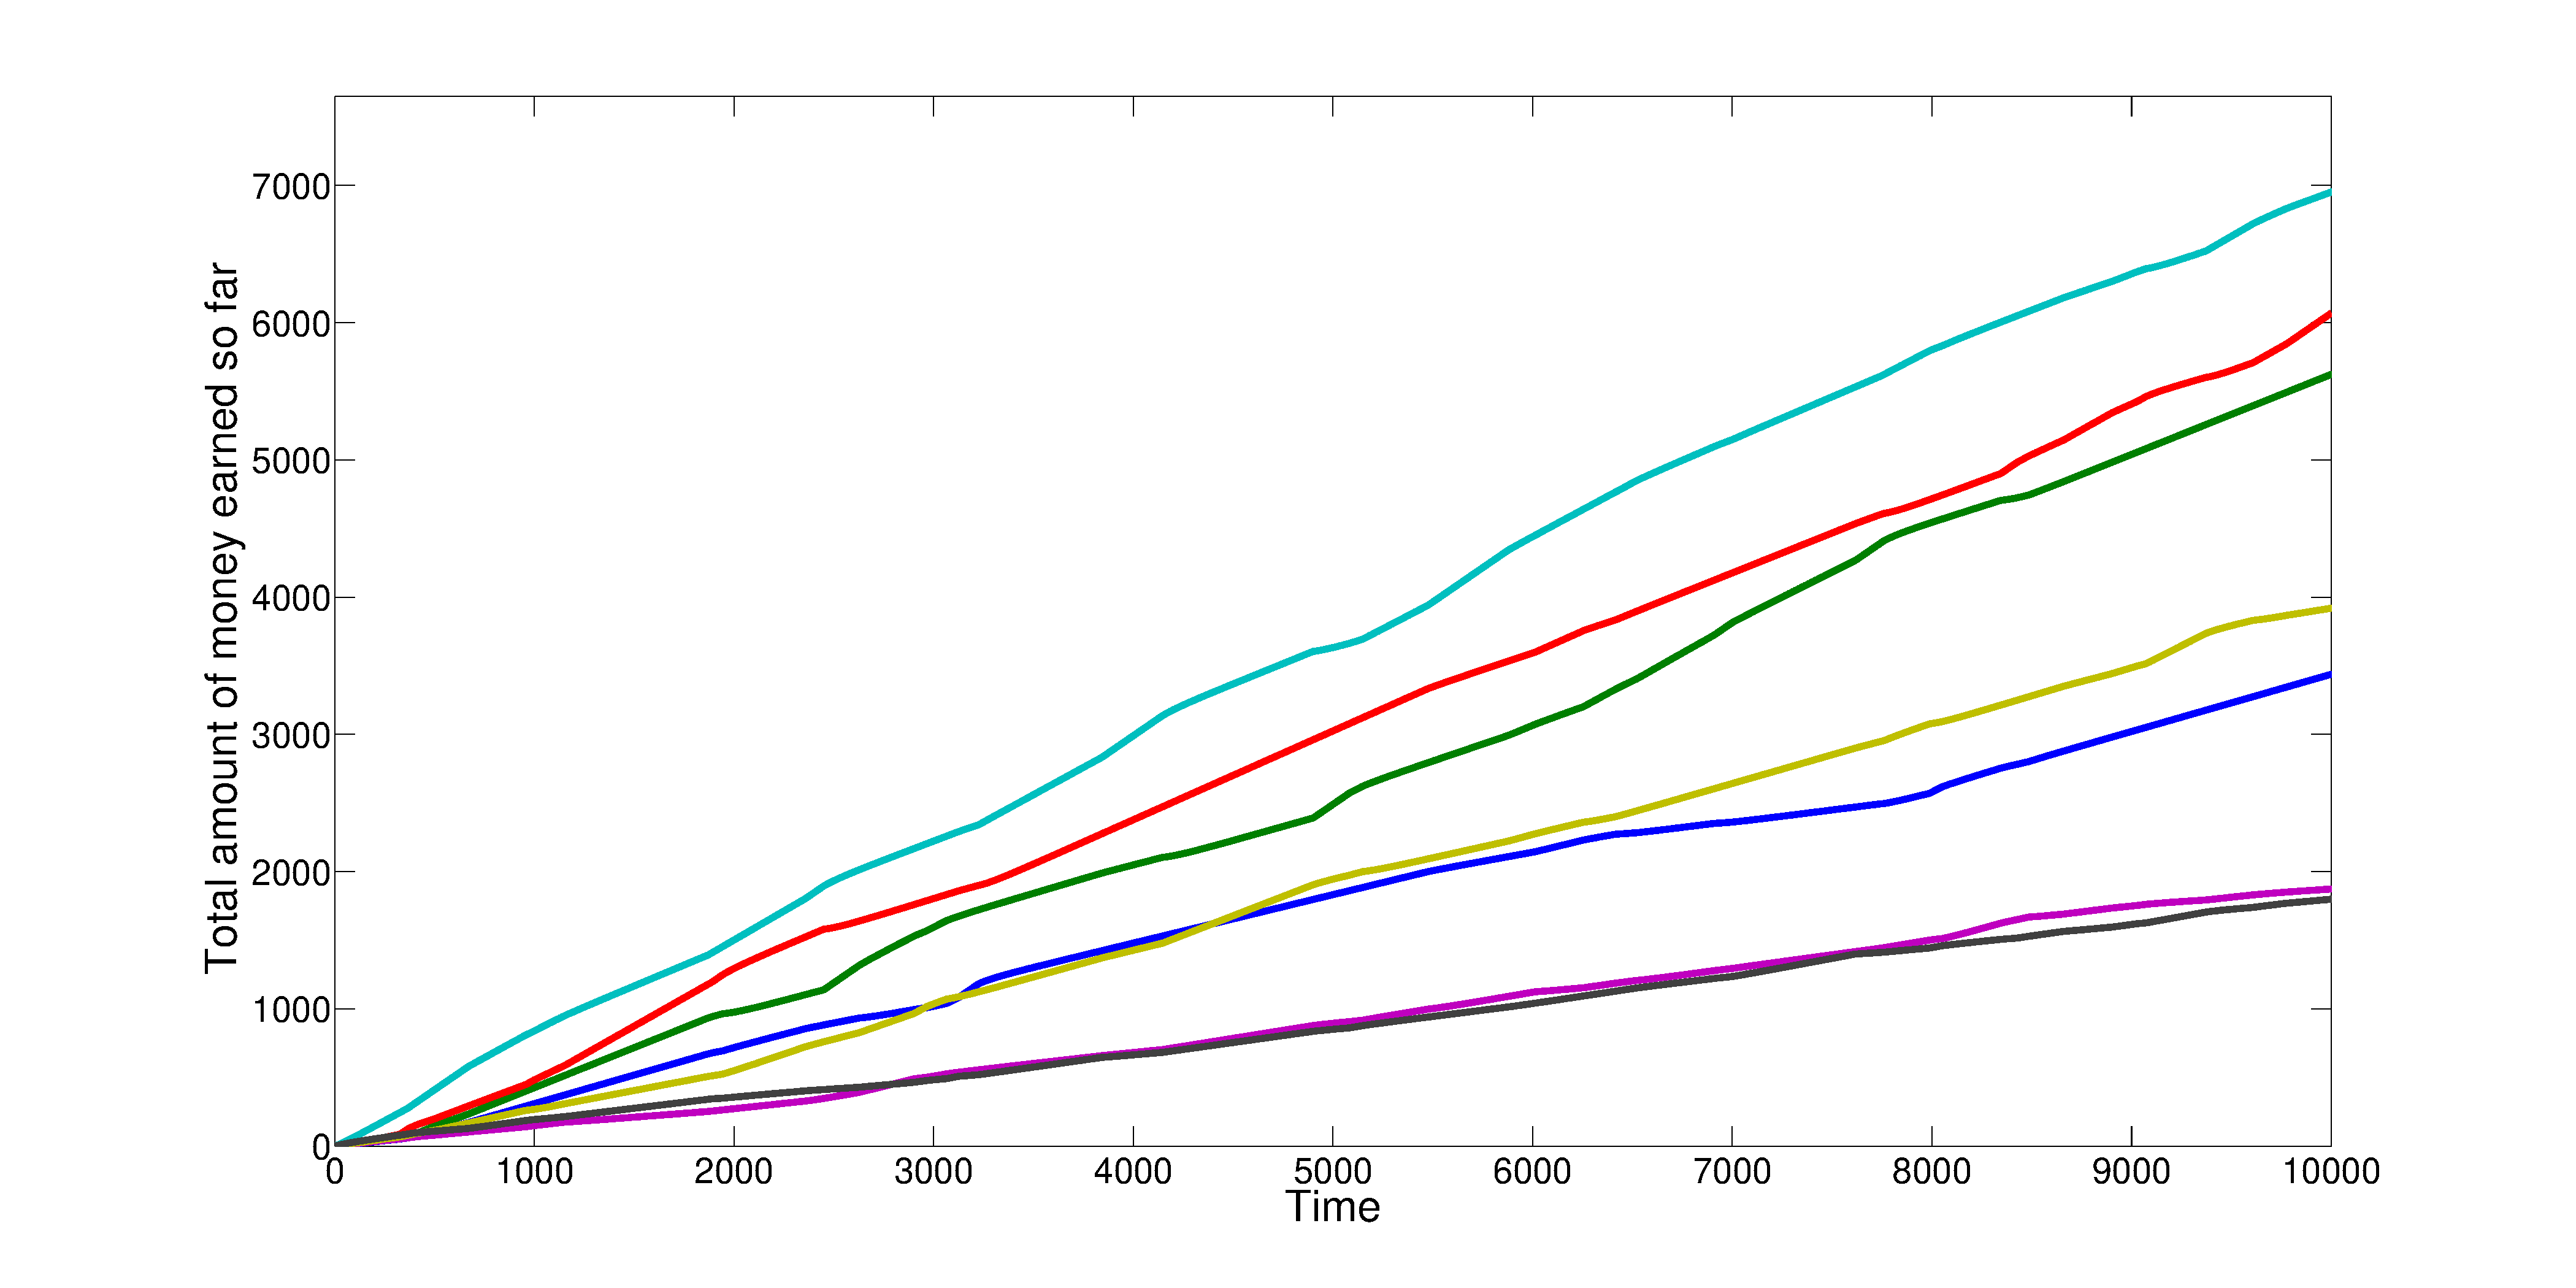
\includegraphics[width=0.9\textwidth]{figures/sd2.pdf}
	\caption{Total money earned by each of the workers. But for $P_\sigma=1.0$ and $A_\sigma=1.4$, the same parameters as in Figure~\ref{fig:sim1totalmoney} were used. The social gap increases a lot and some workers earn several times the salary of other individui.}
	\label{fig:sd2}
\end{figure}
The boredom can be seen as the main reason for choosing a new task. Figure~\ref{fig:noboredom} was obtained by using $\zeta=0$ instead of $\zeta=0.001$ as above. It displays a prompt work specialization, illustrated by the fact that after a short equilibration period, there are no more task changes due to the absence of boredom. 
Figure~\ref{fig:moreboredom1} and \ref{fig:moreboredom2}, on the other hand, were obtained with $\zeta=0.01$ and $B_\mu=1.5$. They show the more frequent task changes and the higher average boredom. It is to be noted that the high sensitivity to boredom in this case does not diminish the social inequalities, which can be seen in Figure~\ref{fig:moreboredom3}. 

The randomness in the generation of $B_{ij}^\textrm{max}$ allows the differenciated sensibility to boredom, which, as mentioned above, has an influence on the rate at which an individual will change tasks.

Another cause for a change in the task is the evolution of the market, meaning that a worker is more likely to leave his current task if a new individuum just joined the new task, thus lowering the average salary.

\begin{figure}[hp!]
	\centering
	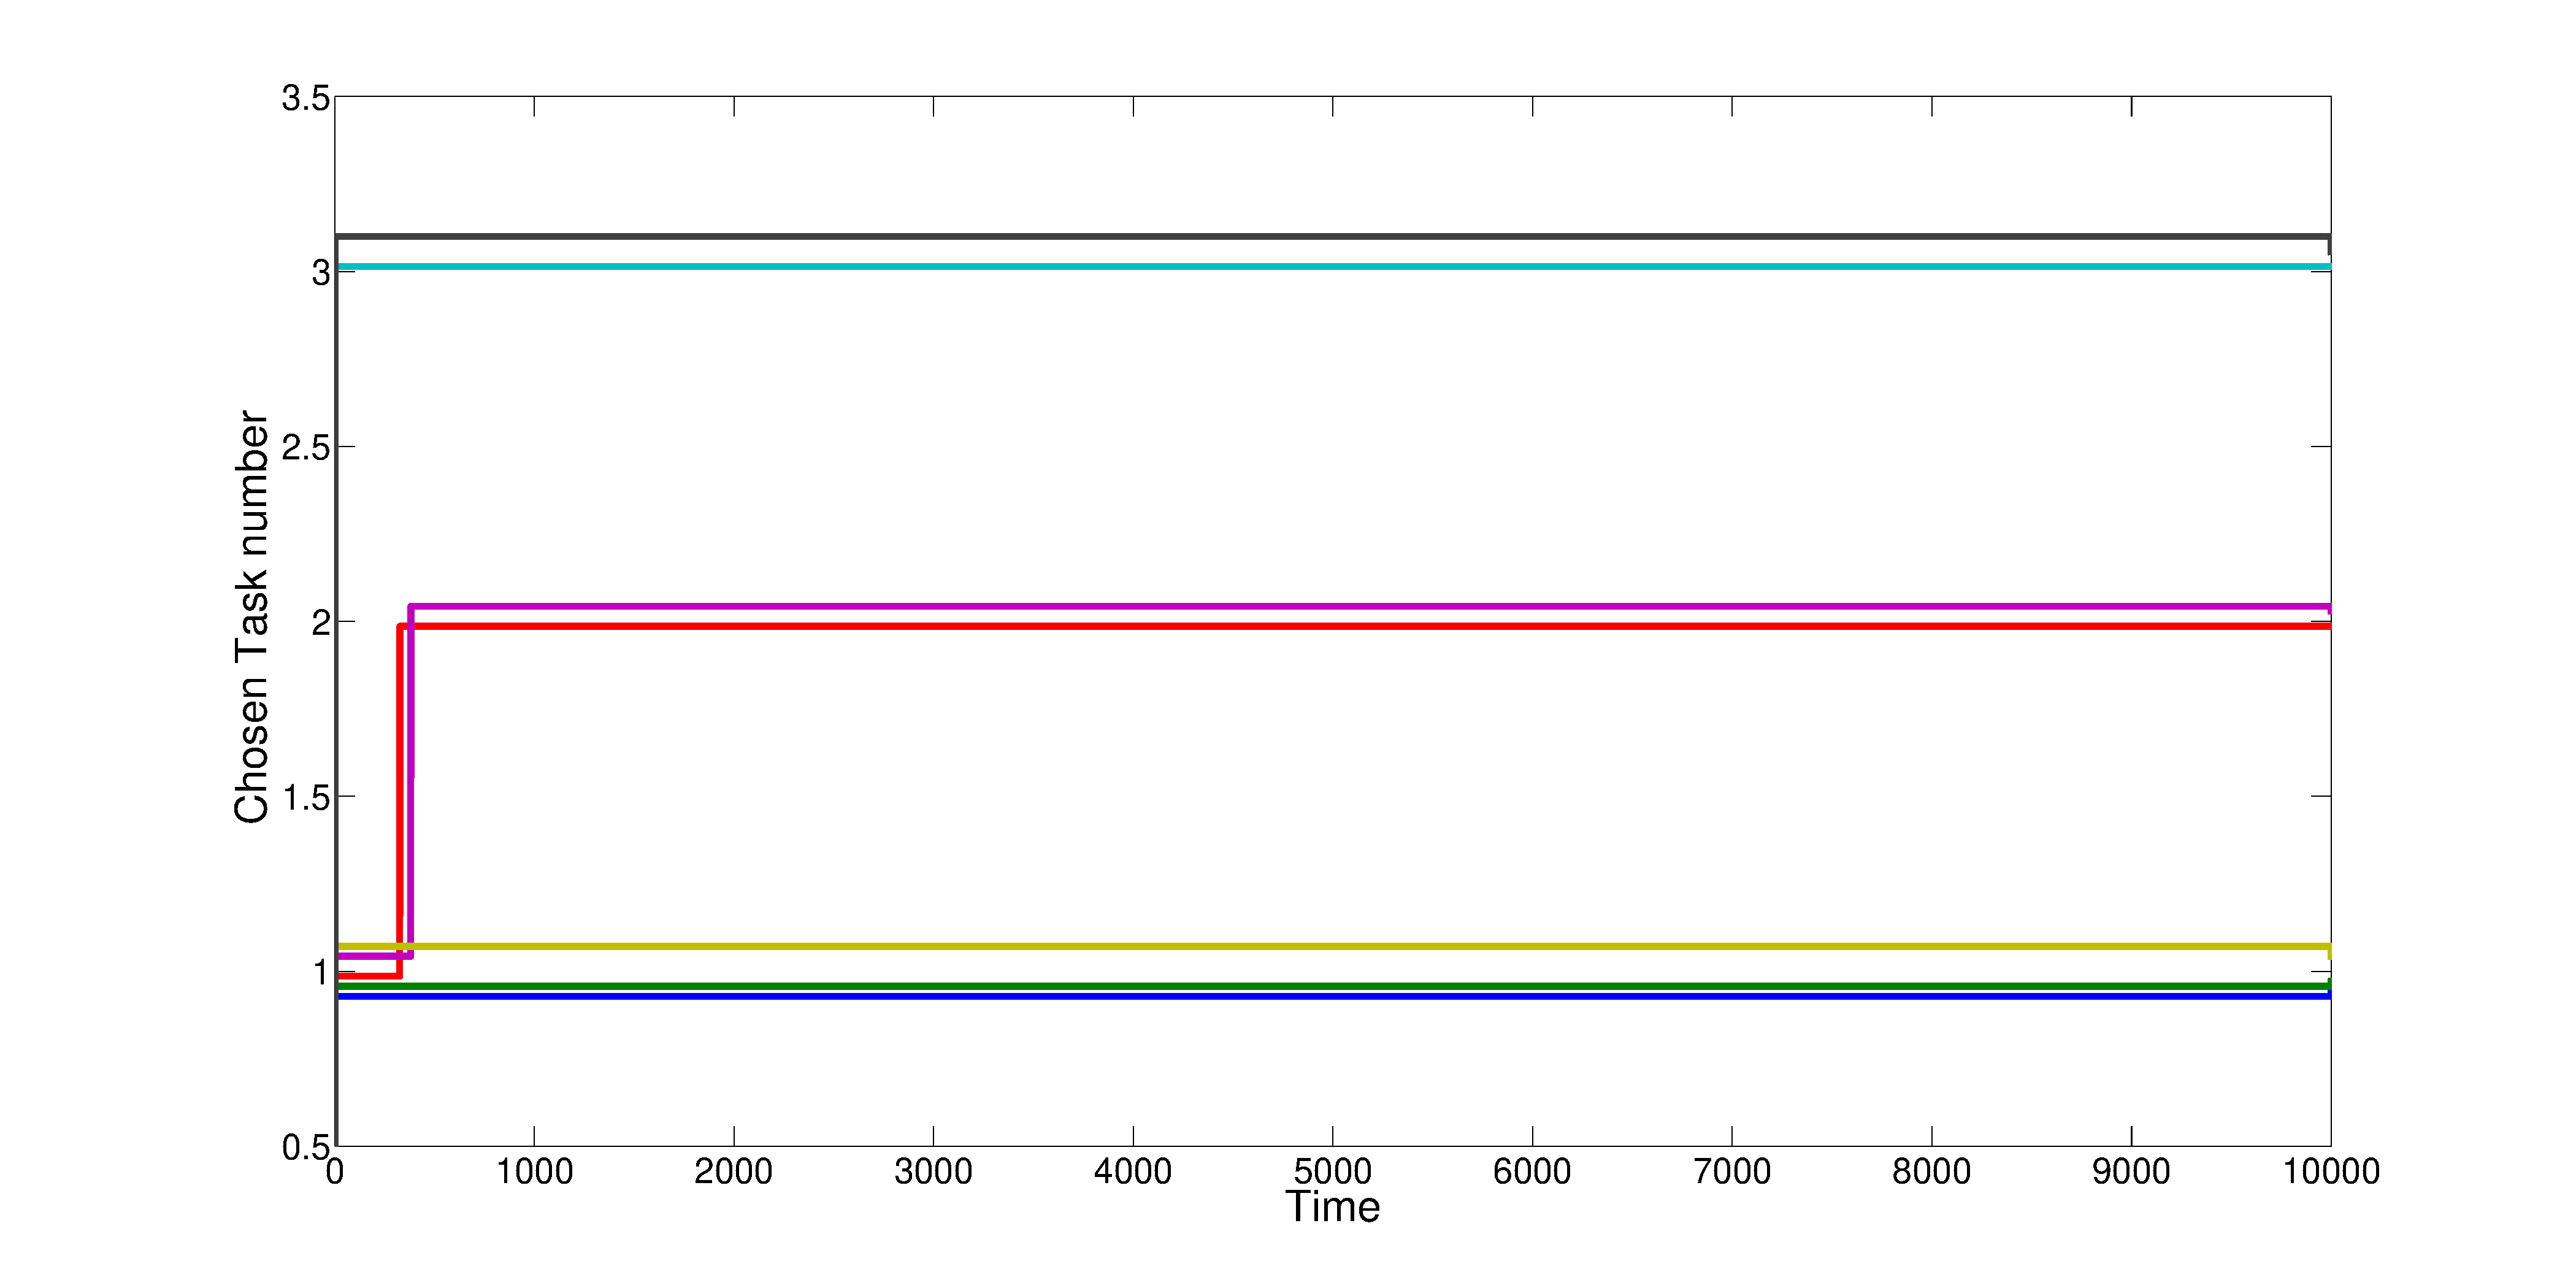
\includegraphics[width=0.9\textwidth]{figures/noboredom.pdf}
	\caption{Chosen task number as a function of time. The same parameters as in Figure~\ref{fig:sim1task} were used but for $\zeta=0$, which implies that the workers do not experience any boredom at all. It shows an early change of task for two of the workers, after which the system does not change anymore.}
	\label{fig:noboredom}
\end{figure}

\begin{figure}[hp!]
	\centering
	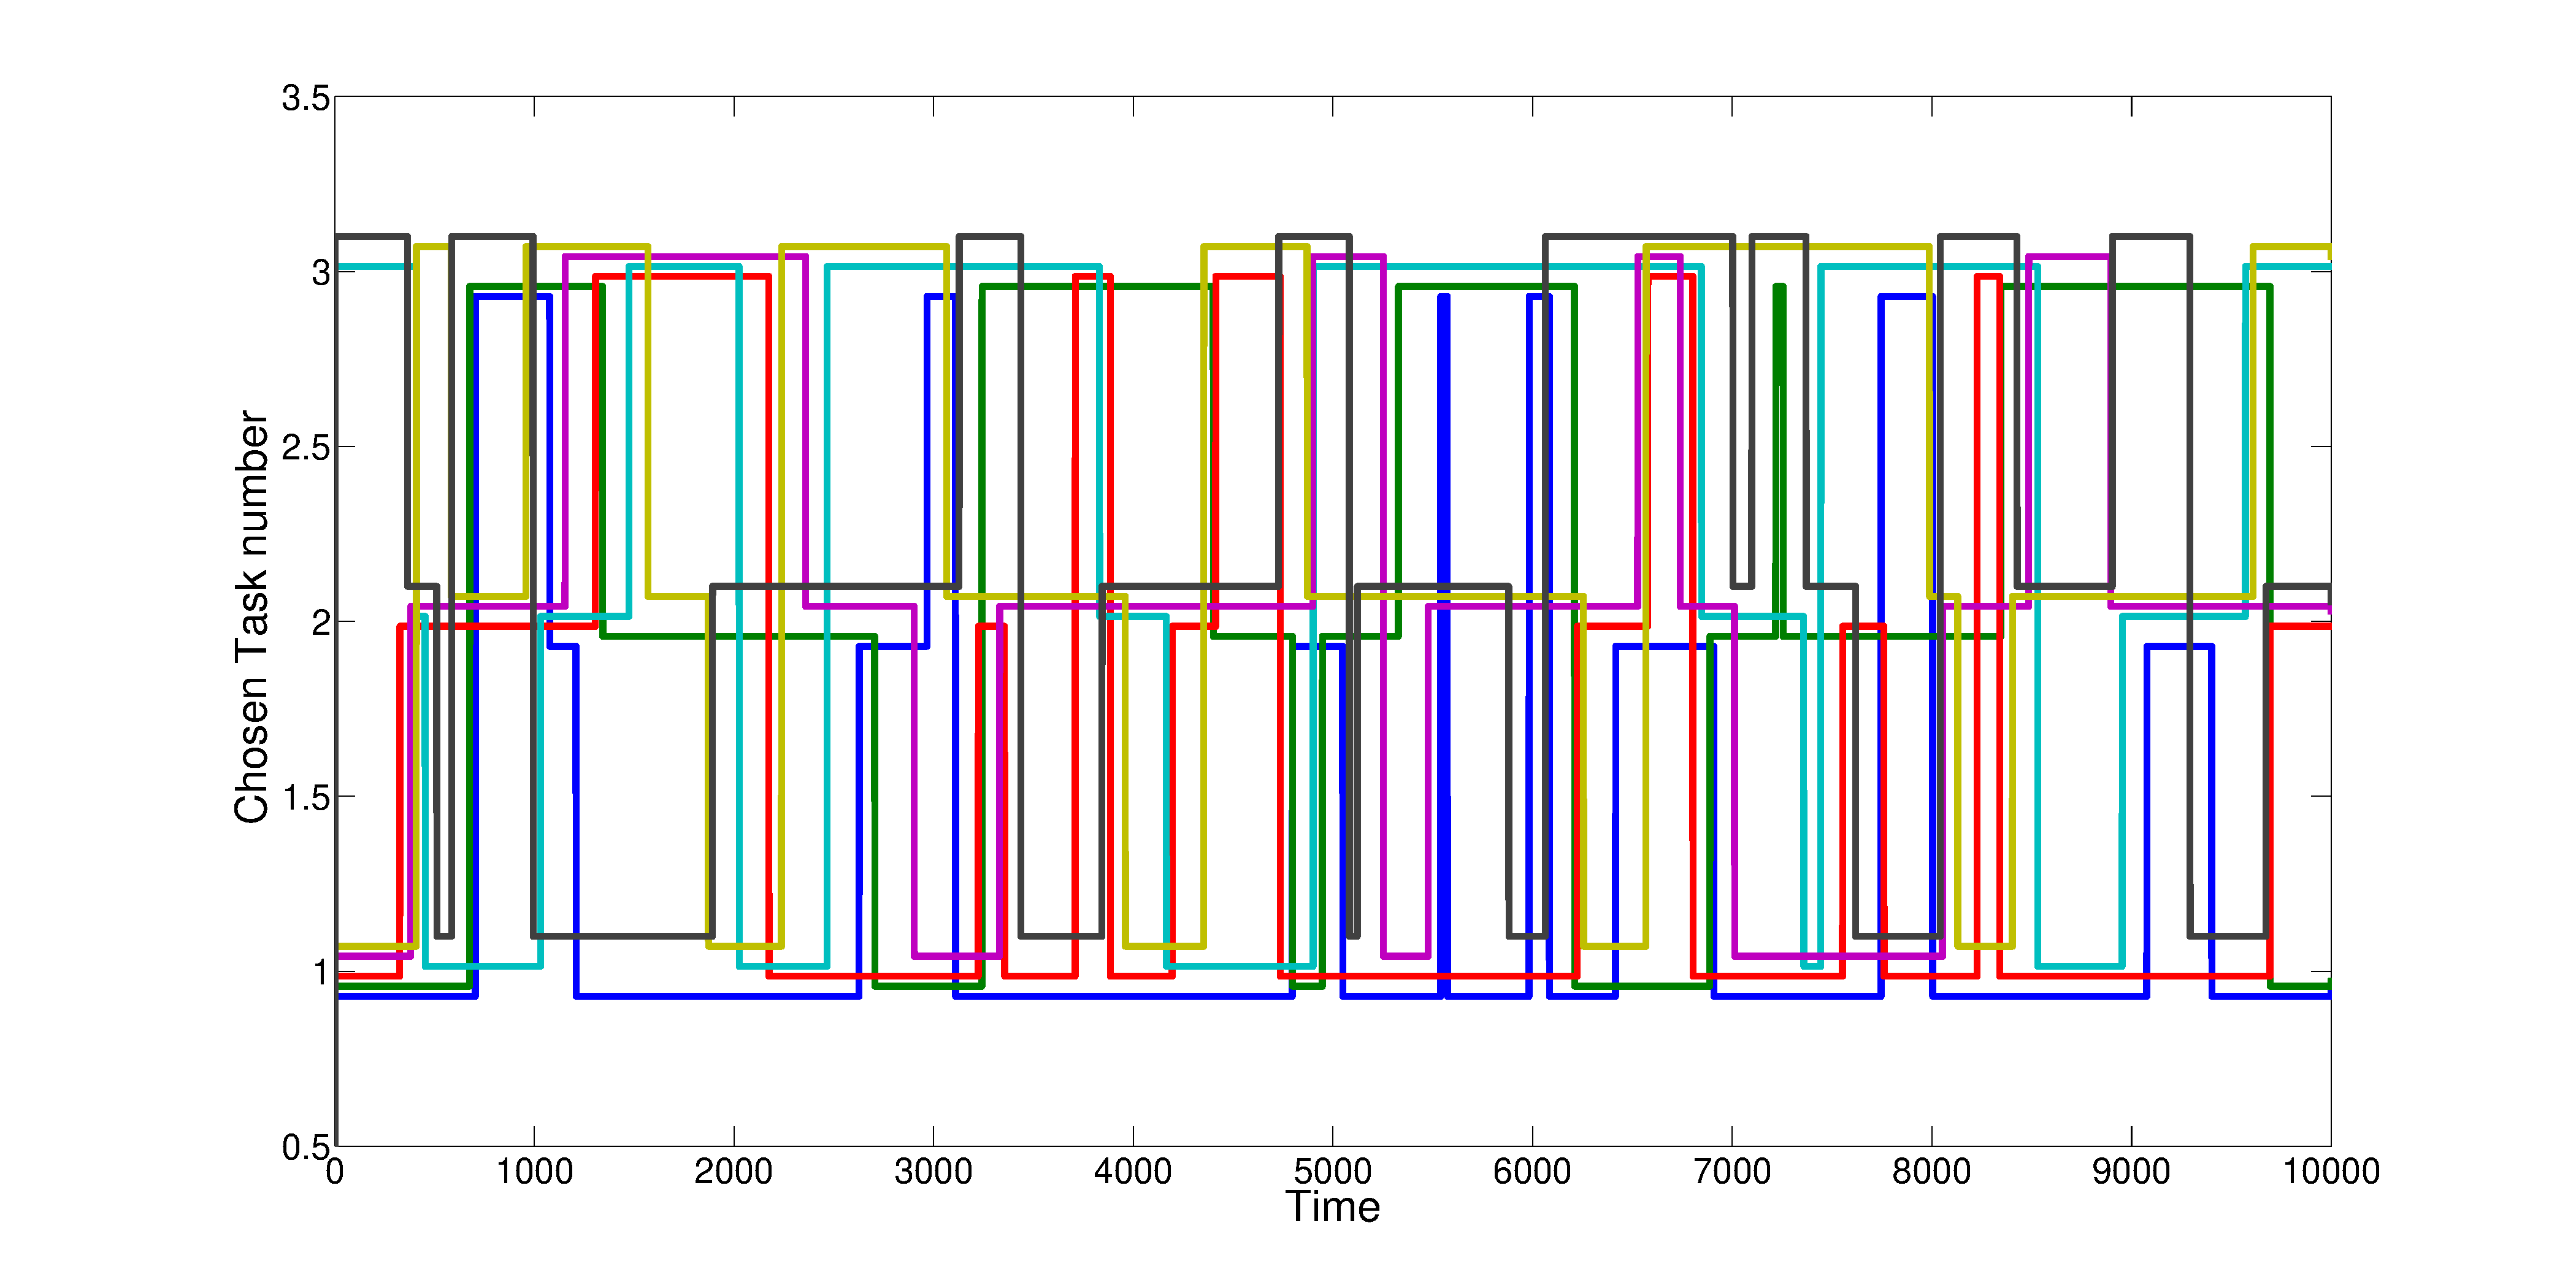
\includegraphics[width=0.9\textwidth]{figures/moreboredom1.pdf}
	\caption{Chosen task number with $\zeta=0.01$ and $B_\mu=1.5$. All the other parameters are the same ones as used for Figure~\ref{fig:sim1task}. The very high rate of task changes is mainly due to the high average boredom, which is displayed in Figure~\ref{fig:moreboredom2}.}
	\label{fig:moreboredom1}
\end{figure}

\begin{figure}[hp!]
	\centering
	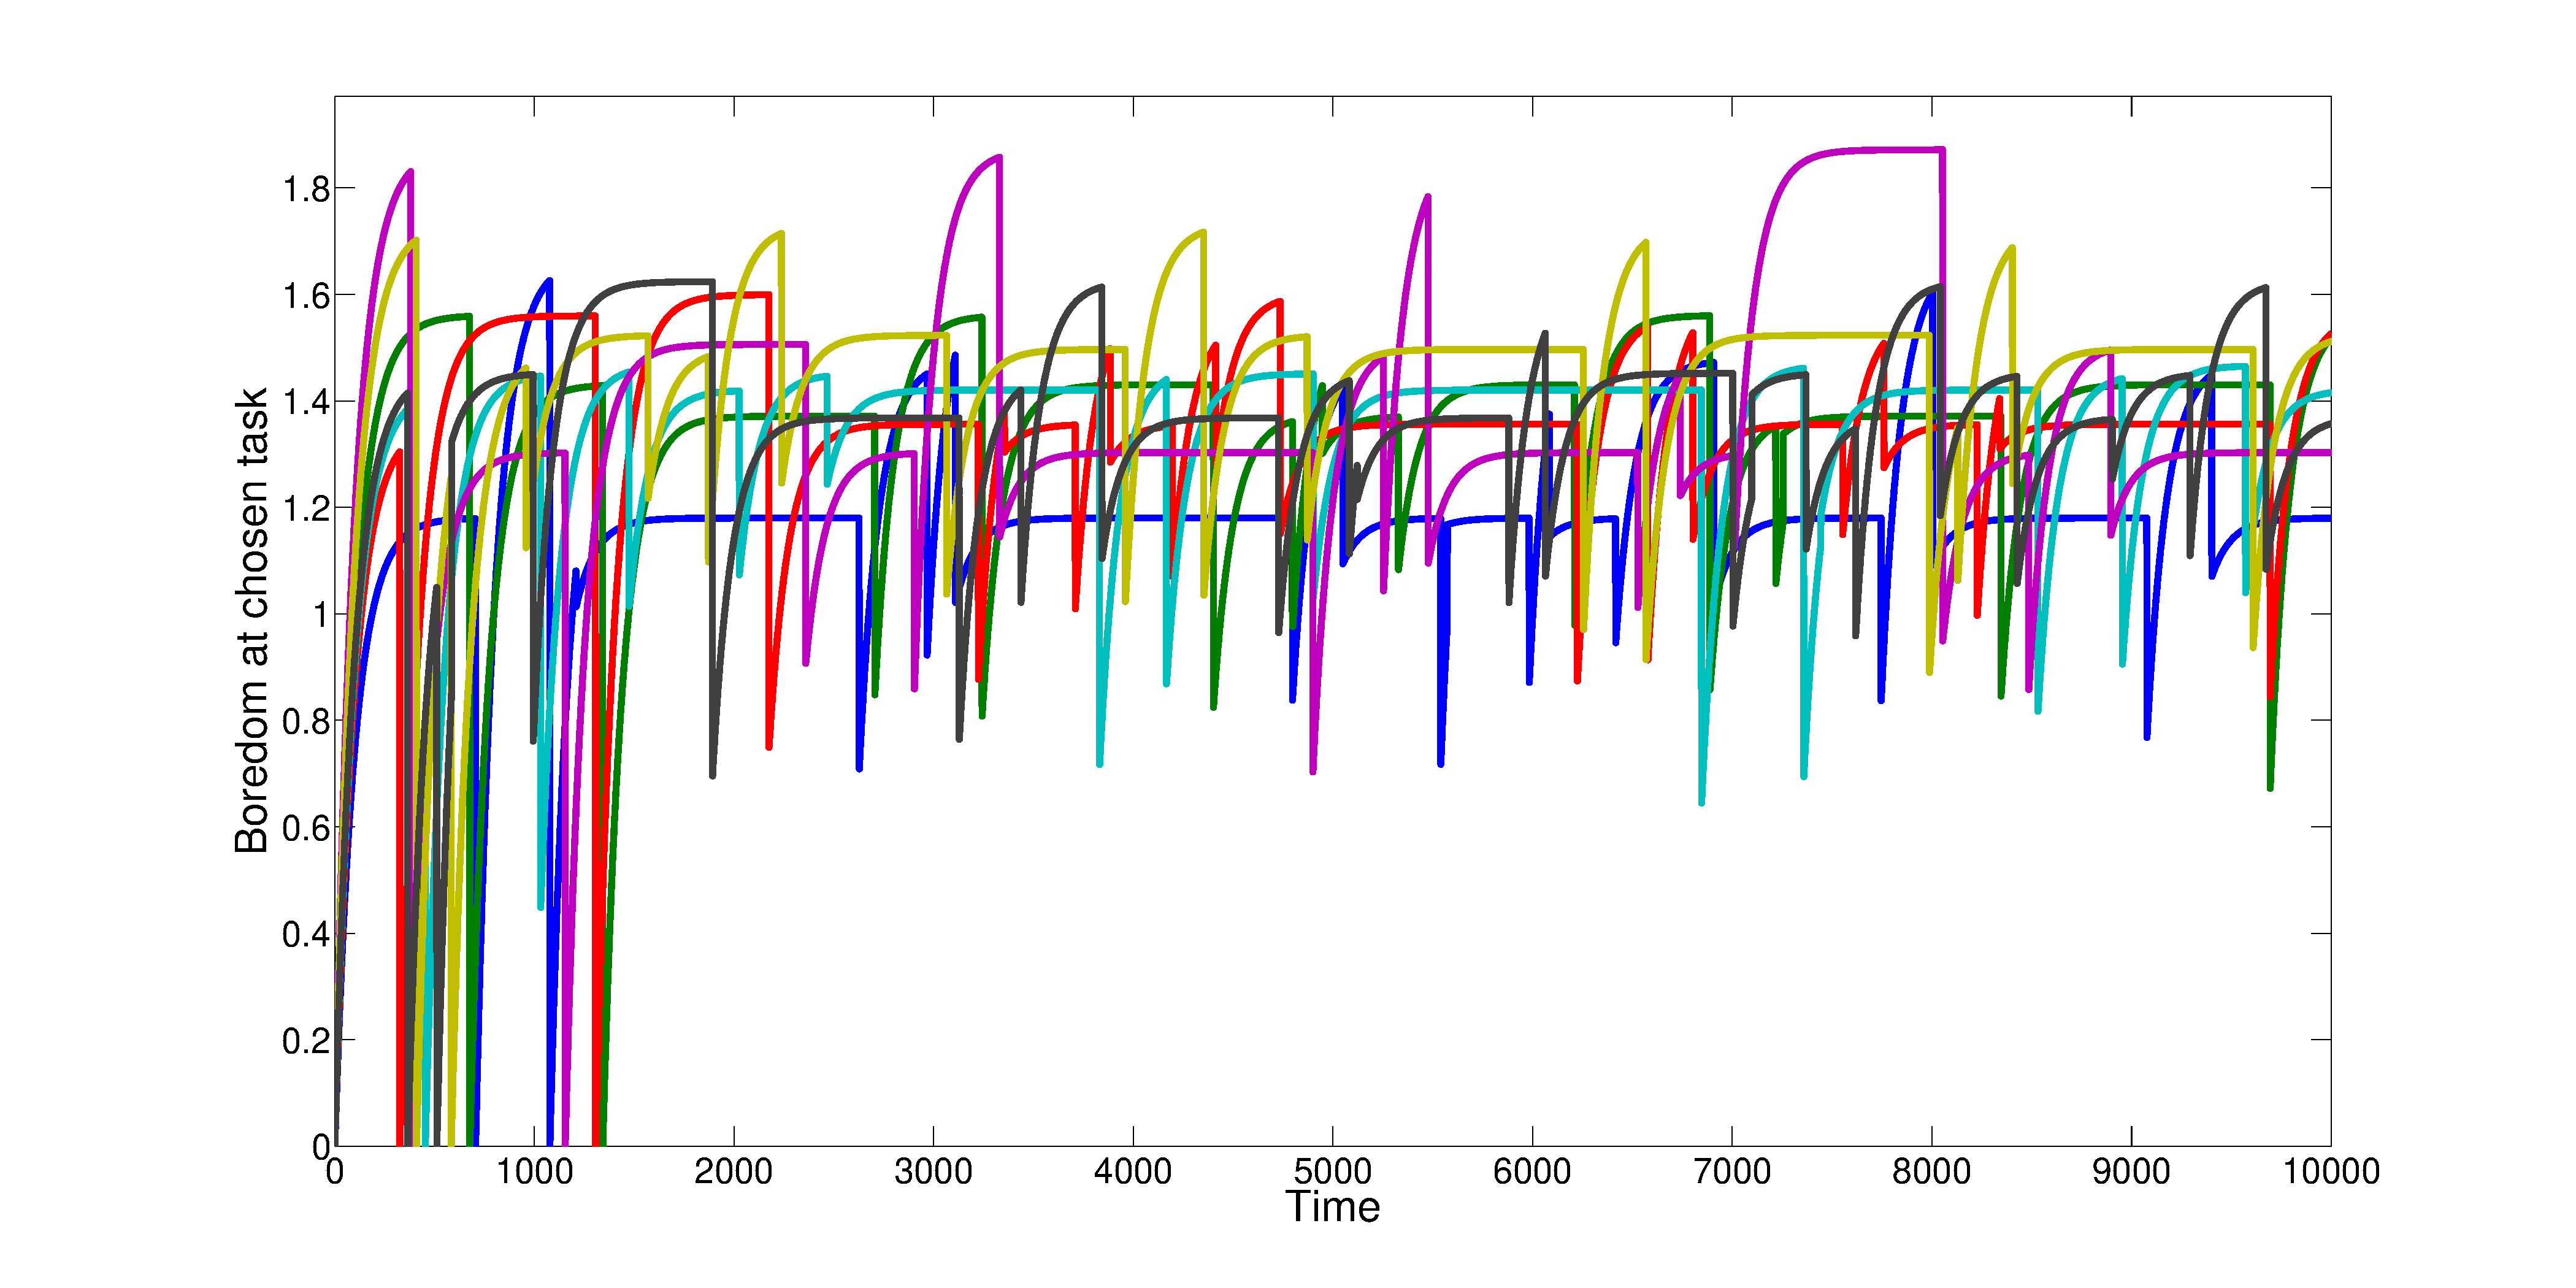
\includegraphics[width=0.9\textwidth]{figures/moreboredom2.pdf}
	\caption{Boredom experienced by the workers at their current task for high maximal boredoms and a high fatigability.}
	\label{fig:moreboredom2}
\end{figure}

\begin{figure}[hp!]
	\centering
	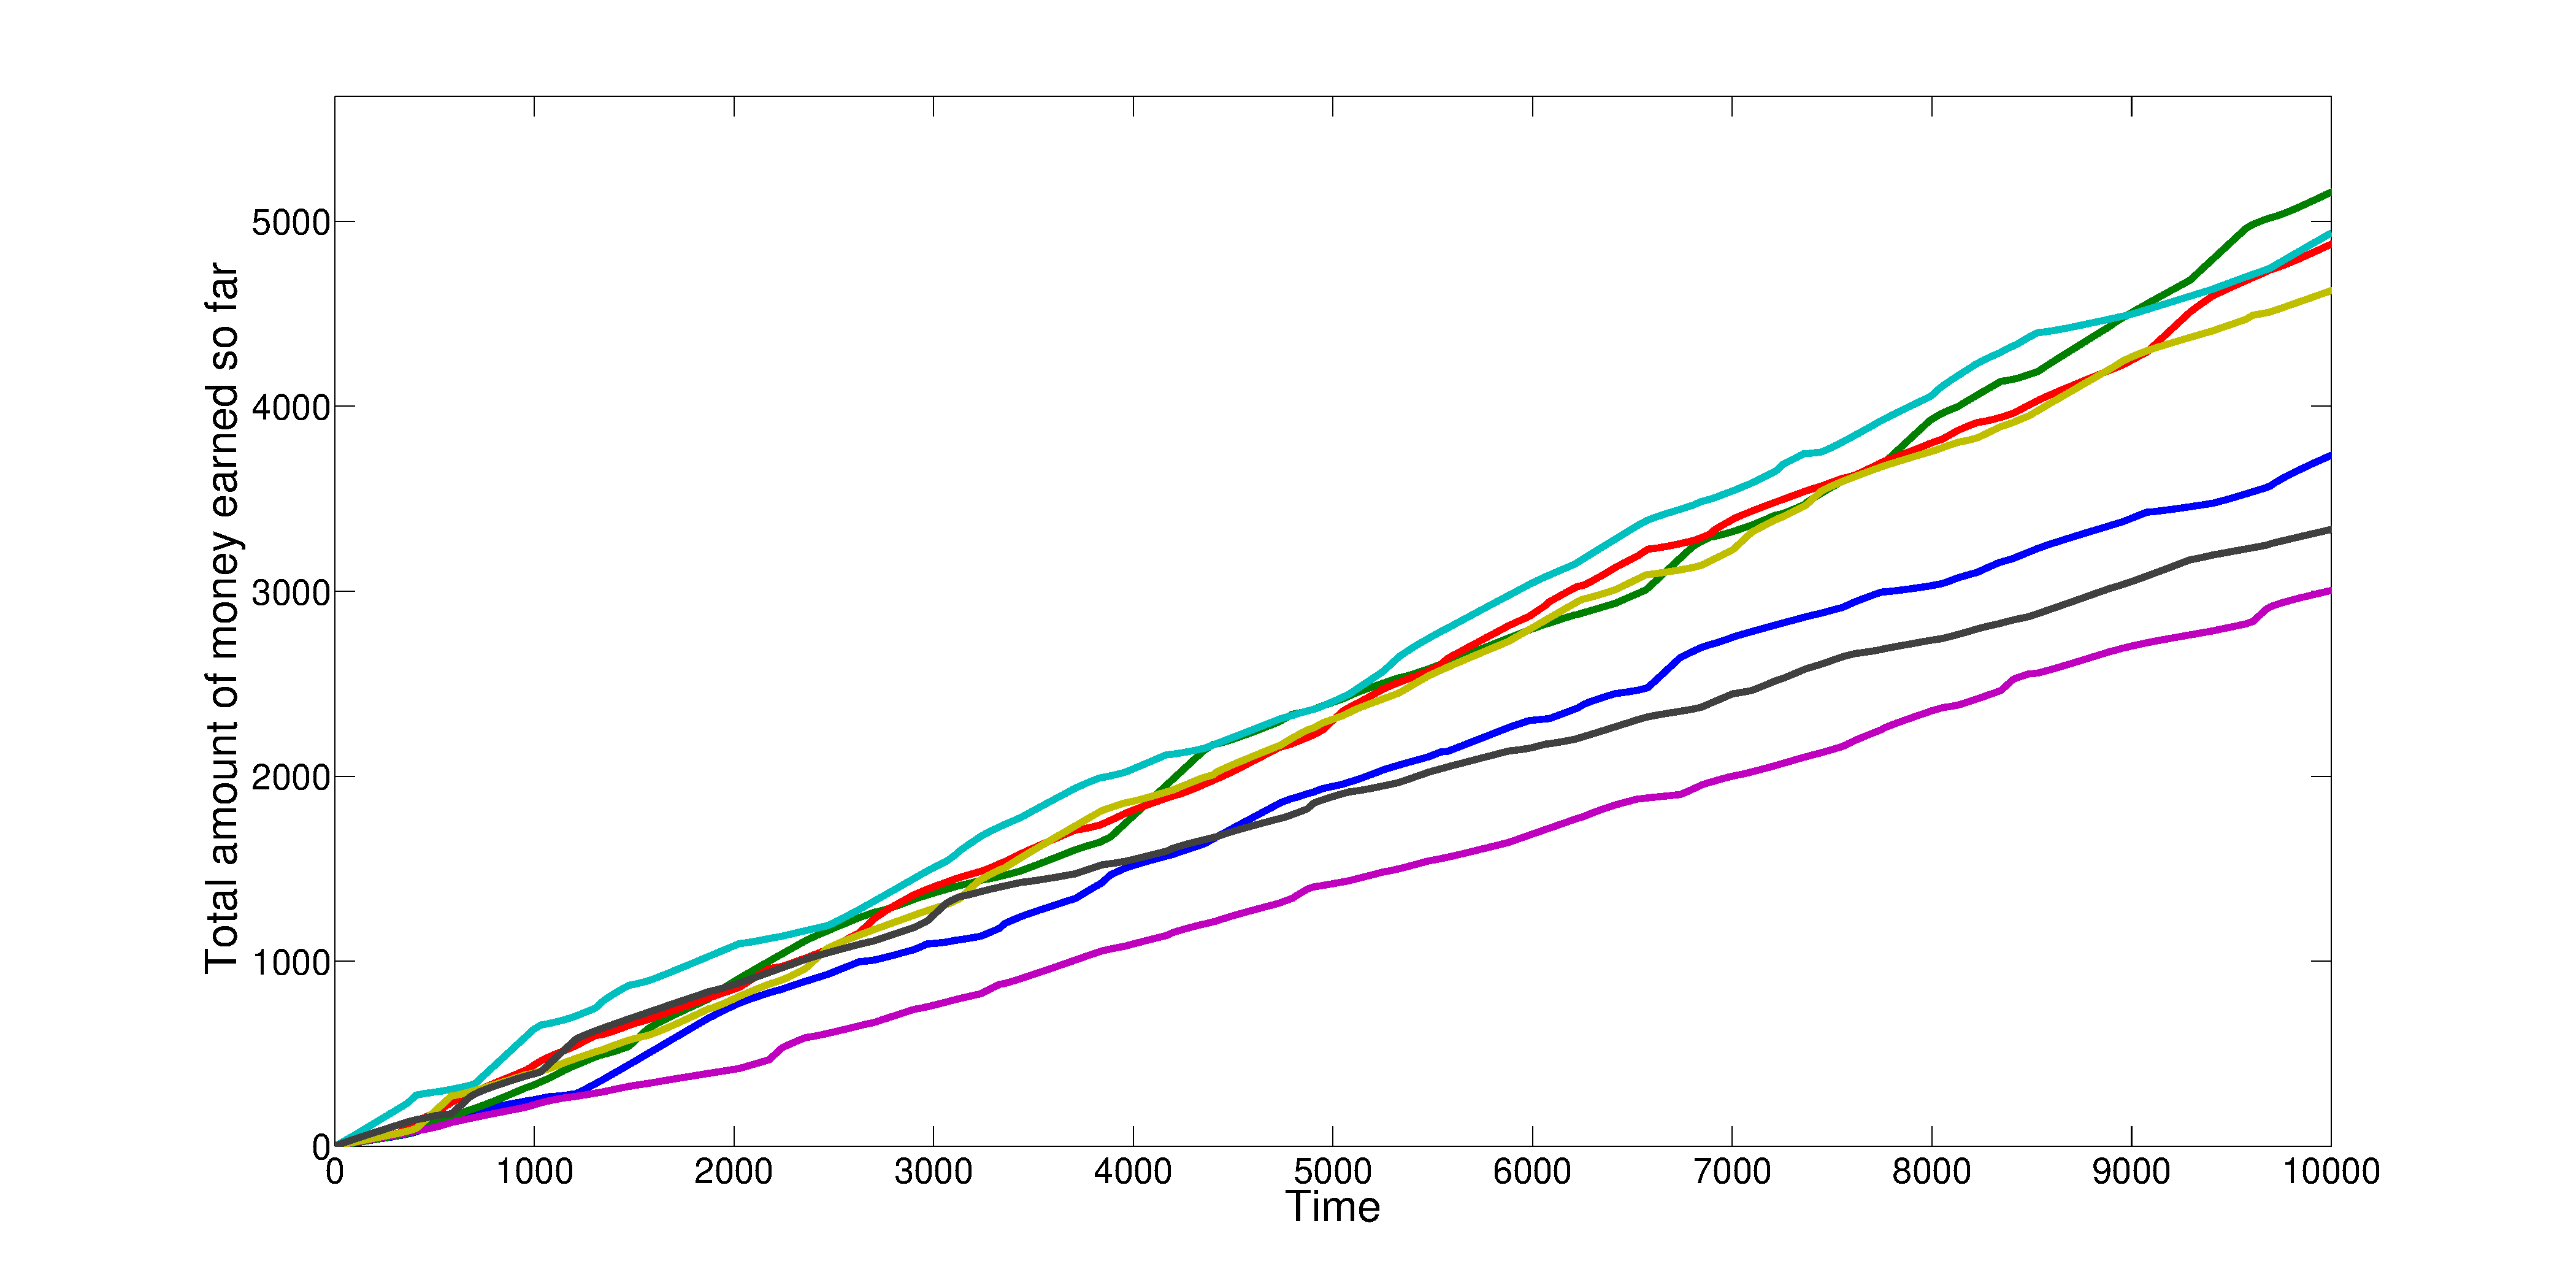
\includegraphics[width=0.9\textwidth]{figures/moreboredom3.pdf}
	\caption{Total amount of money earned by the workers in the case where the fatigability and the maximal boredoms are high. Despite more fluctuations in comparison with Figure~\ref{fig:sim1totalmoney}, the social inequalities are still pronounced.}
	\label{fig:moreboredom3}
\end{figure}

The parameter $p_s$ becomes important when task changes become frequent and a smaller value for $p_s$ will result in less frequent task changes. However, changing $p_s$ above a specific threshold will have a negligible influence, as the additional time a worker has to wait after a new task has become more profitable will change only little.

